\section{Benutzeroberfläche}
%[TODO: remove this link] https://tex.stackexchange.com/questions/442077/is-it-possible-to-use-svg-images-with-overleaf

Es handelt sich hier lediglich um Entwürfe. Dementsprechend sind Änderungen vorbehalten, insbesondere im Design. Auch kann das finale Produkt leicht von diesen Entwürfen abweichen, auch wenn keine größere Änderung vorgenommen wird.\\
Man beachte, das in den Entwürfen auch Funktionalität zu sehen ist, welche aus Wunschkriterien stammen. Die auf diesen Entwürfen enthaltenen Markierungen (Kreise mit Zahlen und rotem Rand) dienen lediglich zur Lokalisierung der Erläuterungen und werden nicht im final Entwurf enthalten sein.
\subsection{Anmeldung}
\label{pages:login}
\begin{figure}[H]
    \centering
    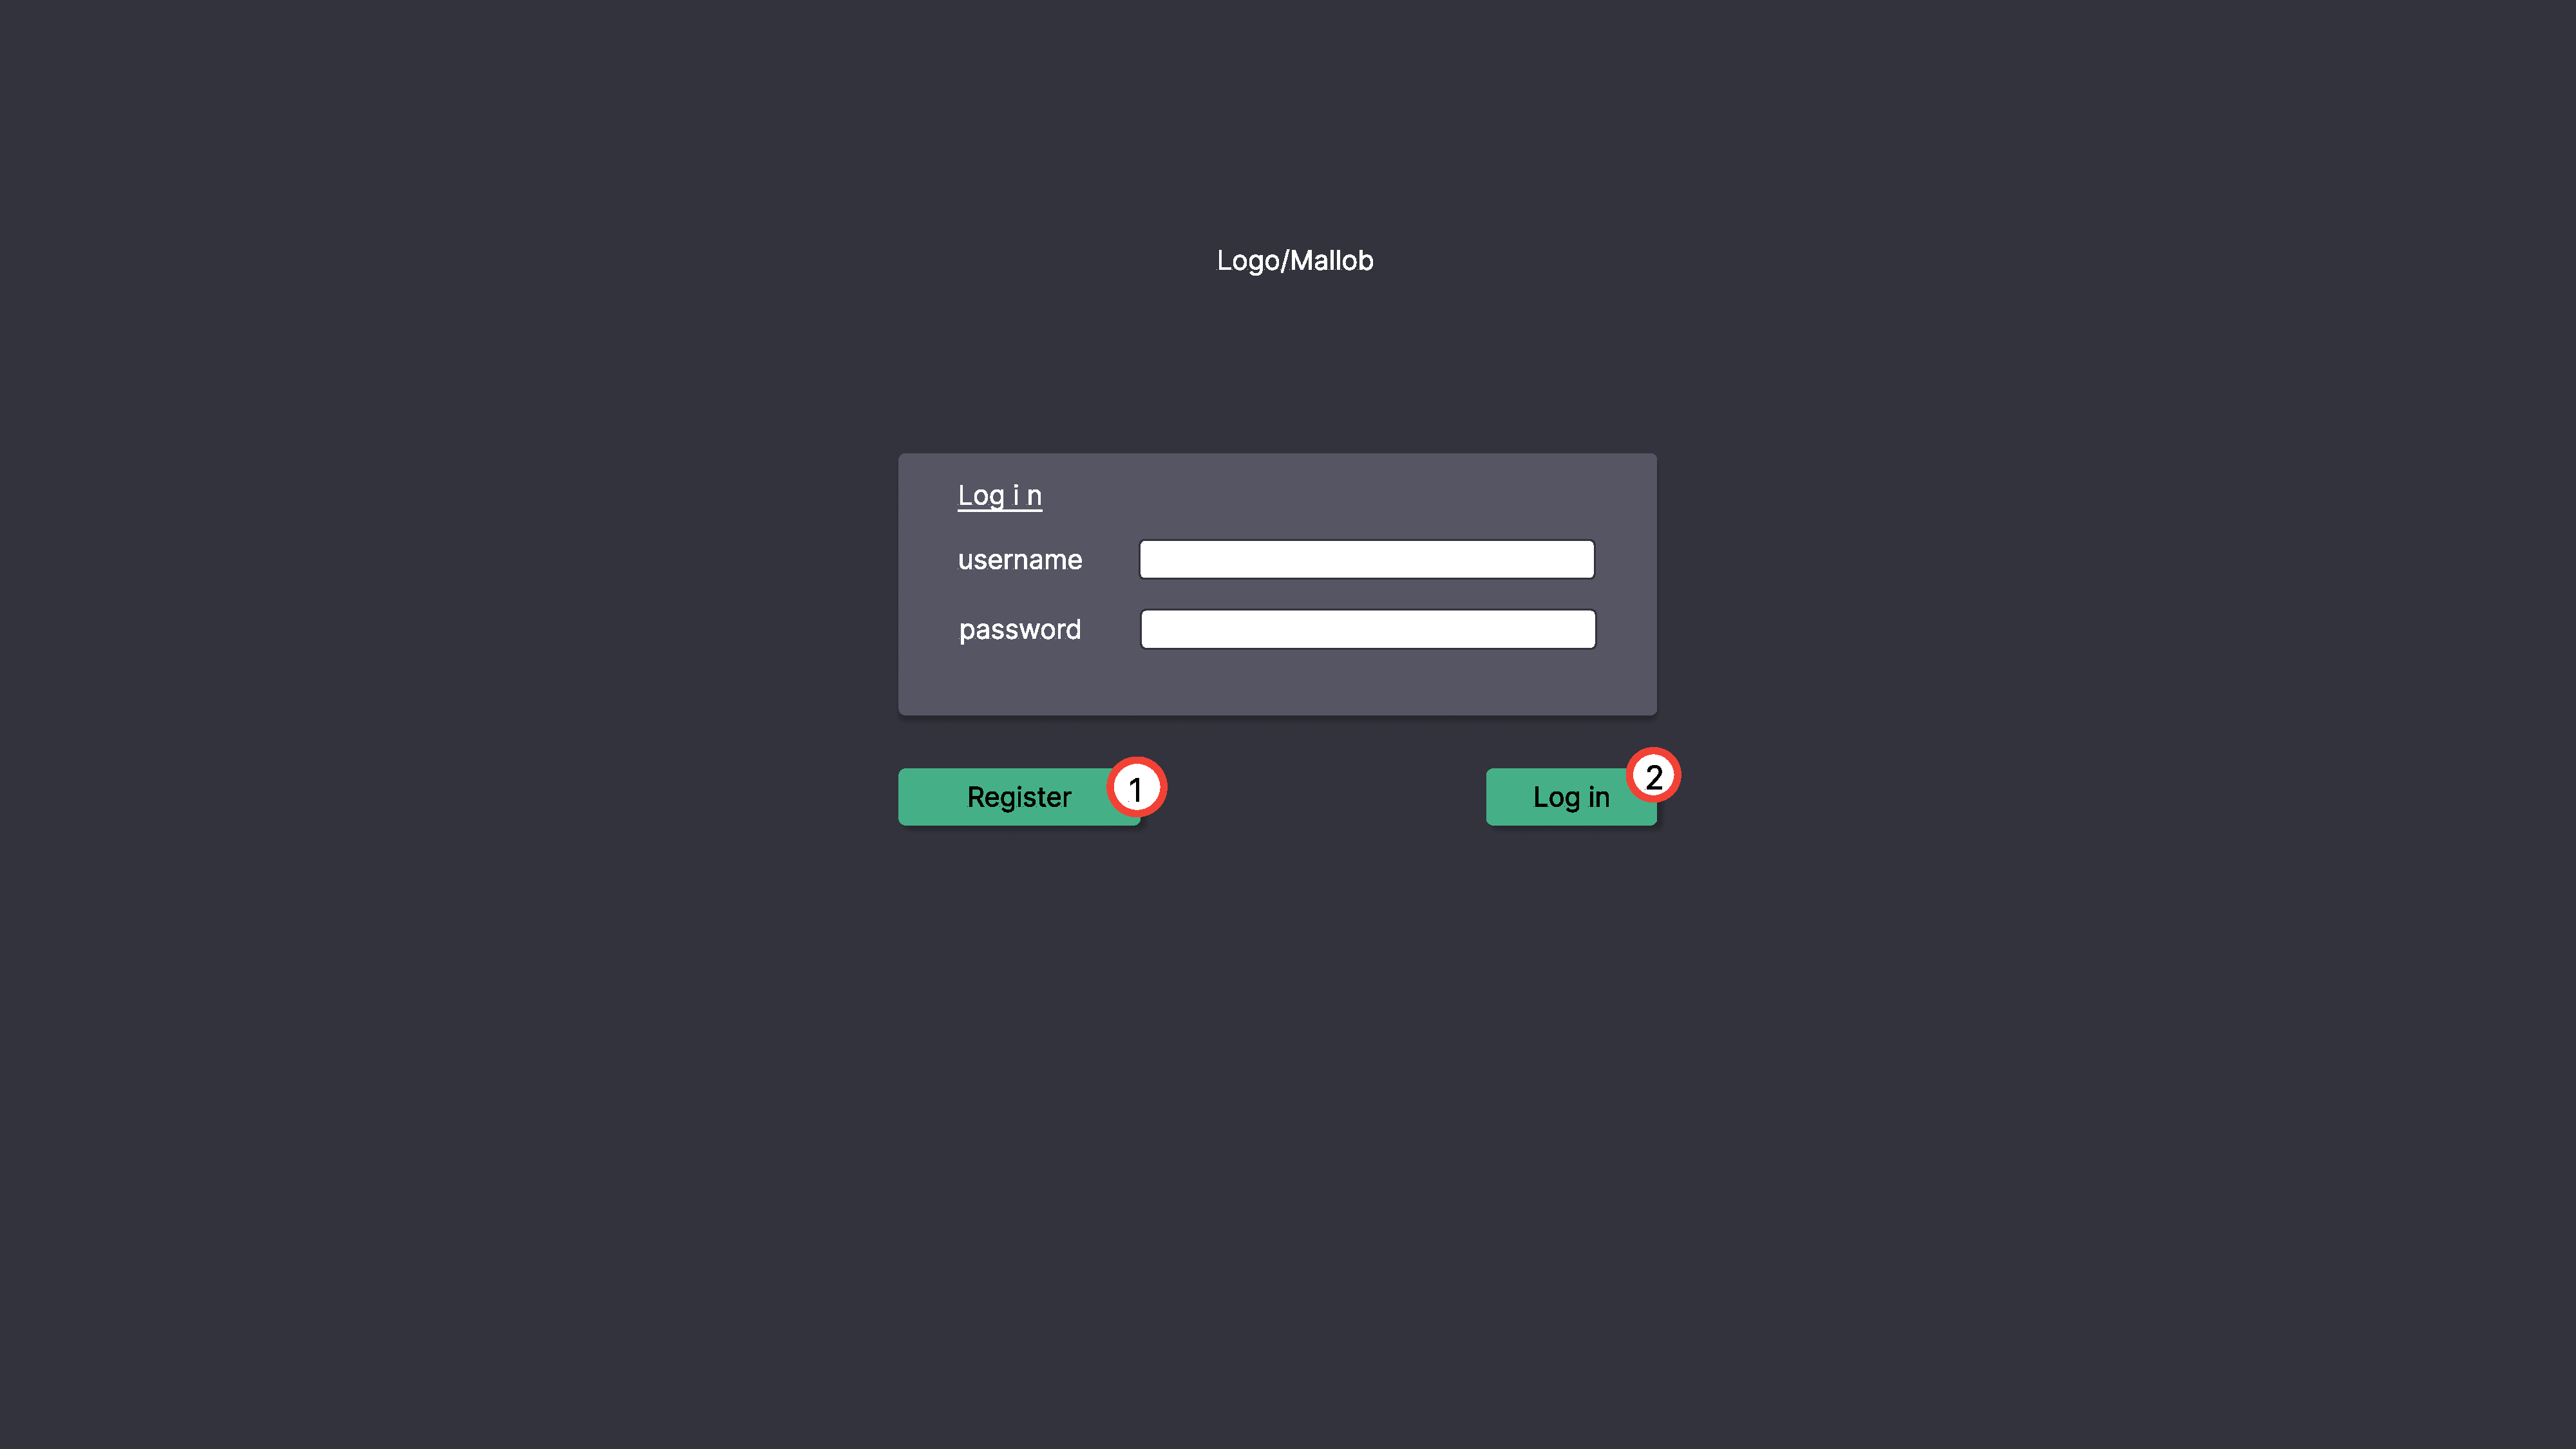
\includegraphics[width=\textwidth]{images-interface/v3_interface/login_page_v3.pdf}
    \caption{Anmeldung}
    \label{fig:login}
\end{figure}
\textbf{Erläuterungen}
\begin{itemize}
    \item[1)] Die Schaltfläche \enquote{Register} leitet zur \hyperref[pages:register]{Registrierungsseite} weiter.
    \item[2)] Die Schaltfläche \enquote{Log in} meldet den Nutzer bei korrekt eingegebenen Daten an und leitet ihn zur \hyperref[pages:job-table]{Job-Tabelle} weiter.
\end{itemize}

\newpage
\subsection{Registrierung}
\label{pages:register}
\begin{figure}[H]
    \centering
    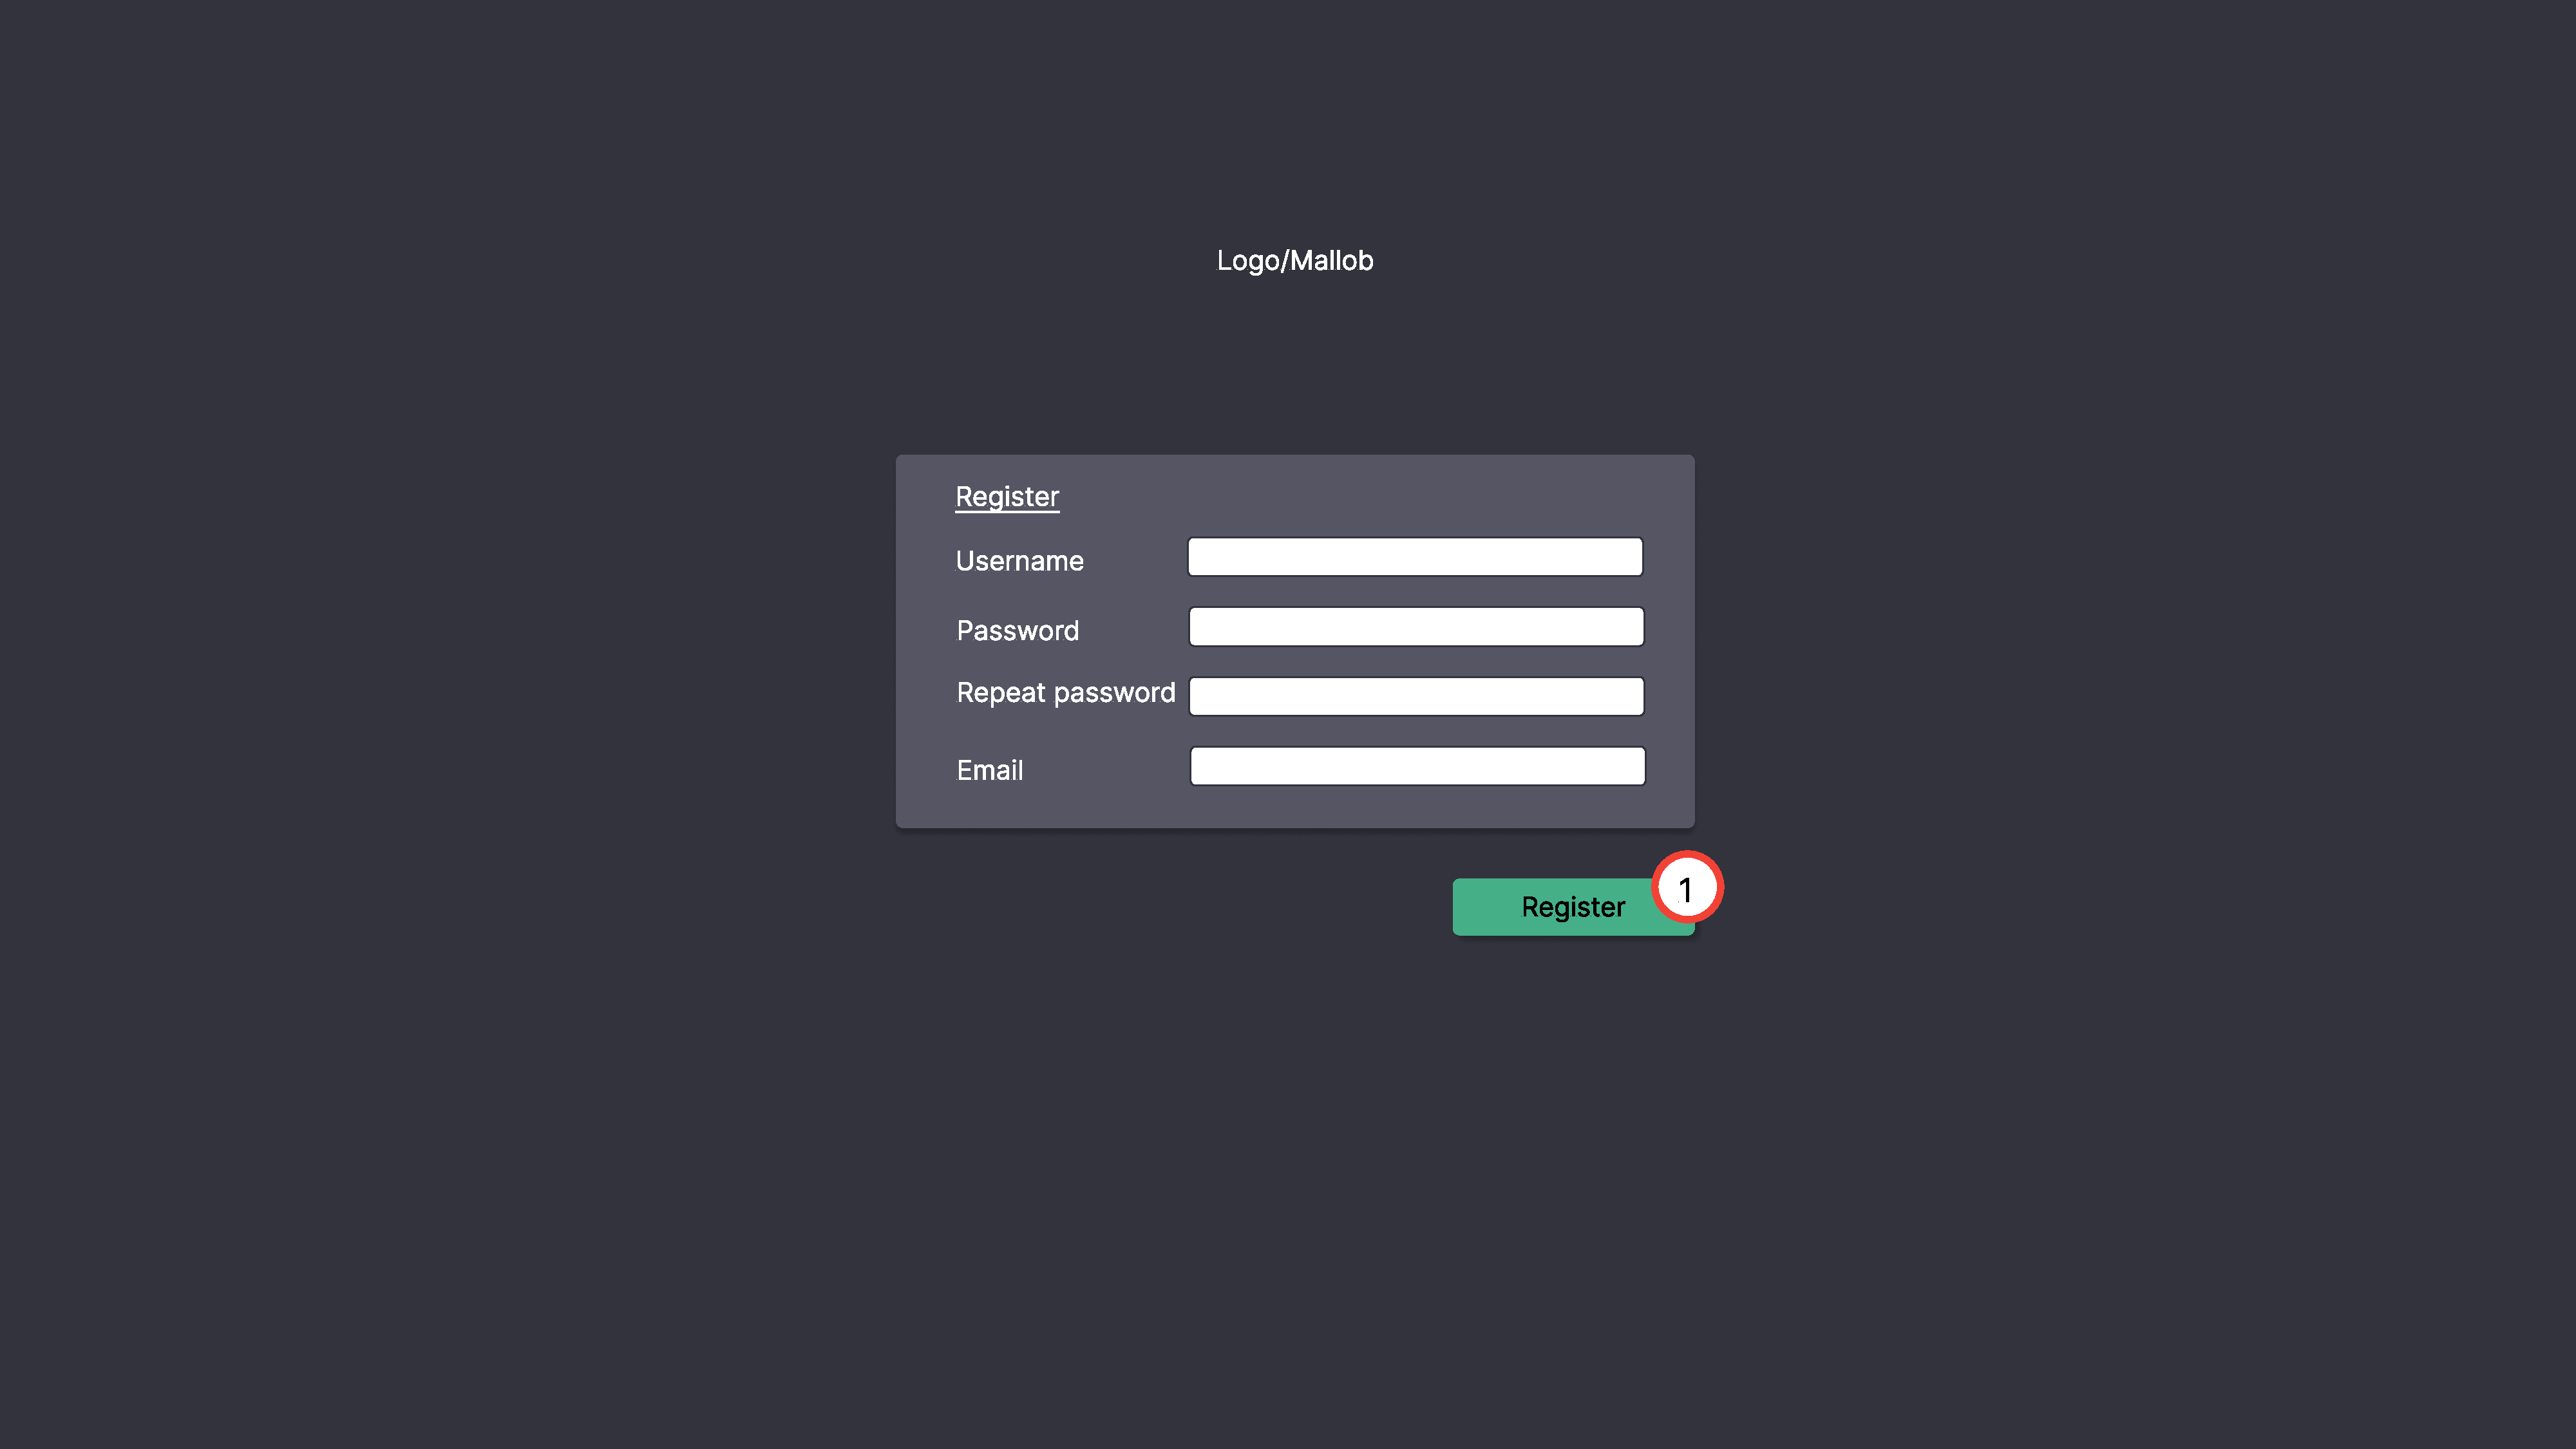
\includegraphics[width=\textwidth]{images-interface/v3_interface/register_page_v3.pdf}
    \caption{Registrierung}
    \label{fig:register}
\end{figure}
\textbf{Erläuterungen}
\begin{itemize}
    \item[1)] Die Schaltfläche \enquote{Register} registriert den Nutzer und leitet in zur \hyperref[pages:visualization]{Visualisierung} weiter, da sein Konto direkt nach der Registrierung noch nicht verifiziert ist und er somit ohnehin noch keine Jobs einreichen kann.
\end{itemize}



\newpage
\subsection{Job-Tabelle}
\label{pages:job-table}
\begin{figure}[H]
    \centering
    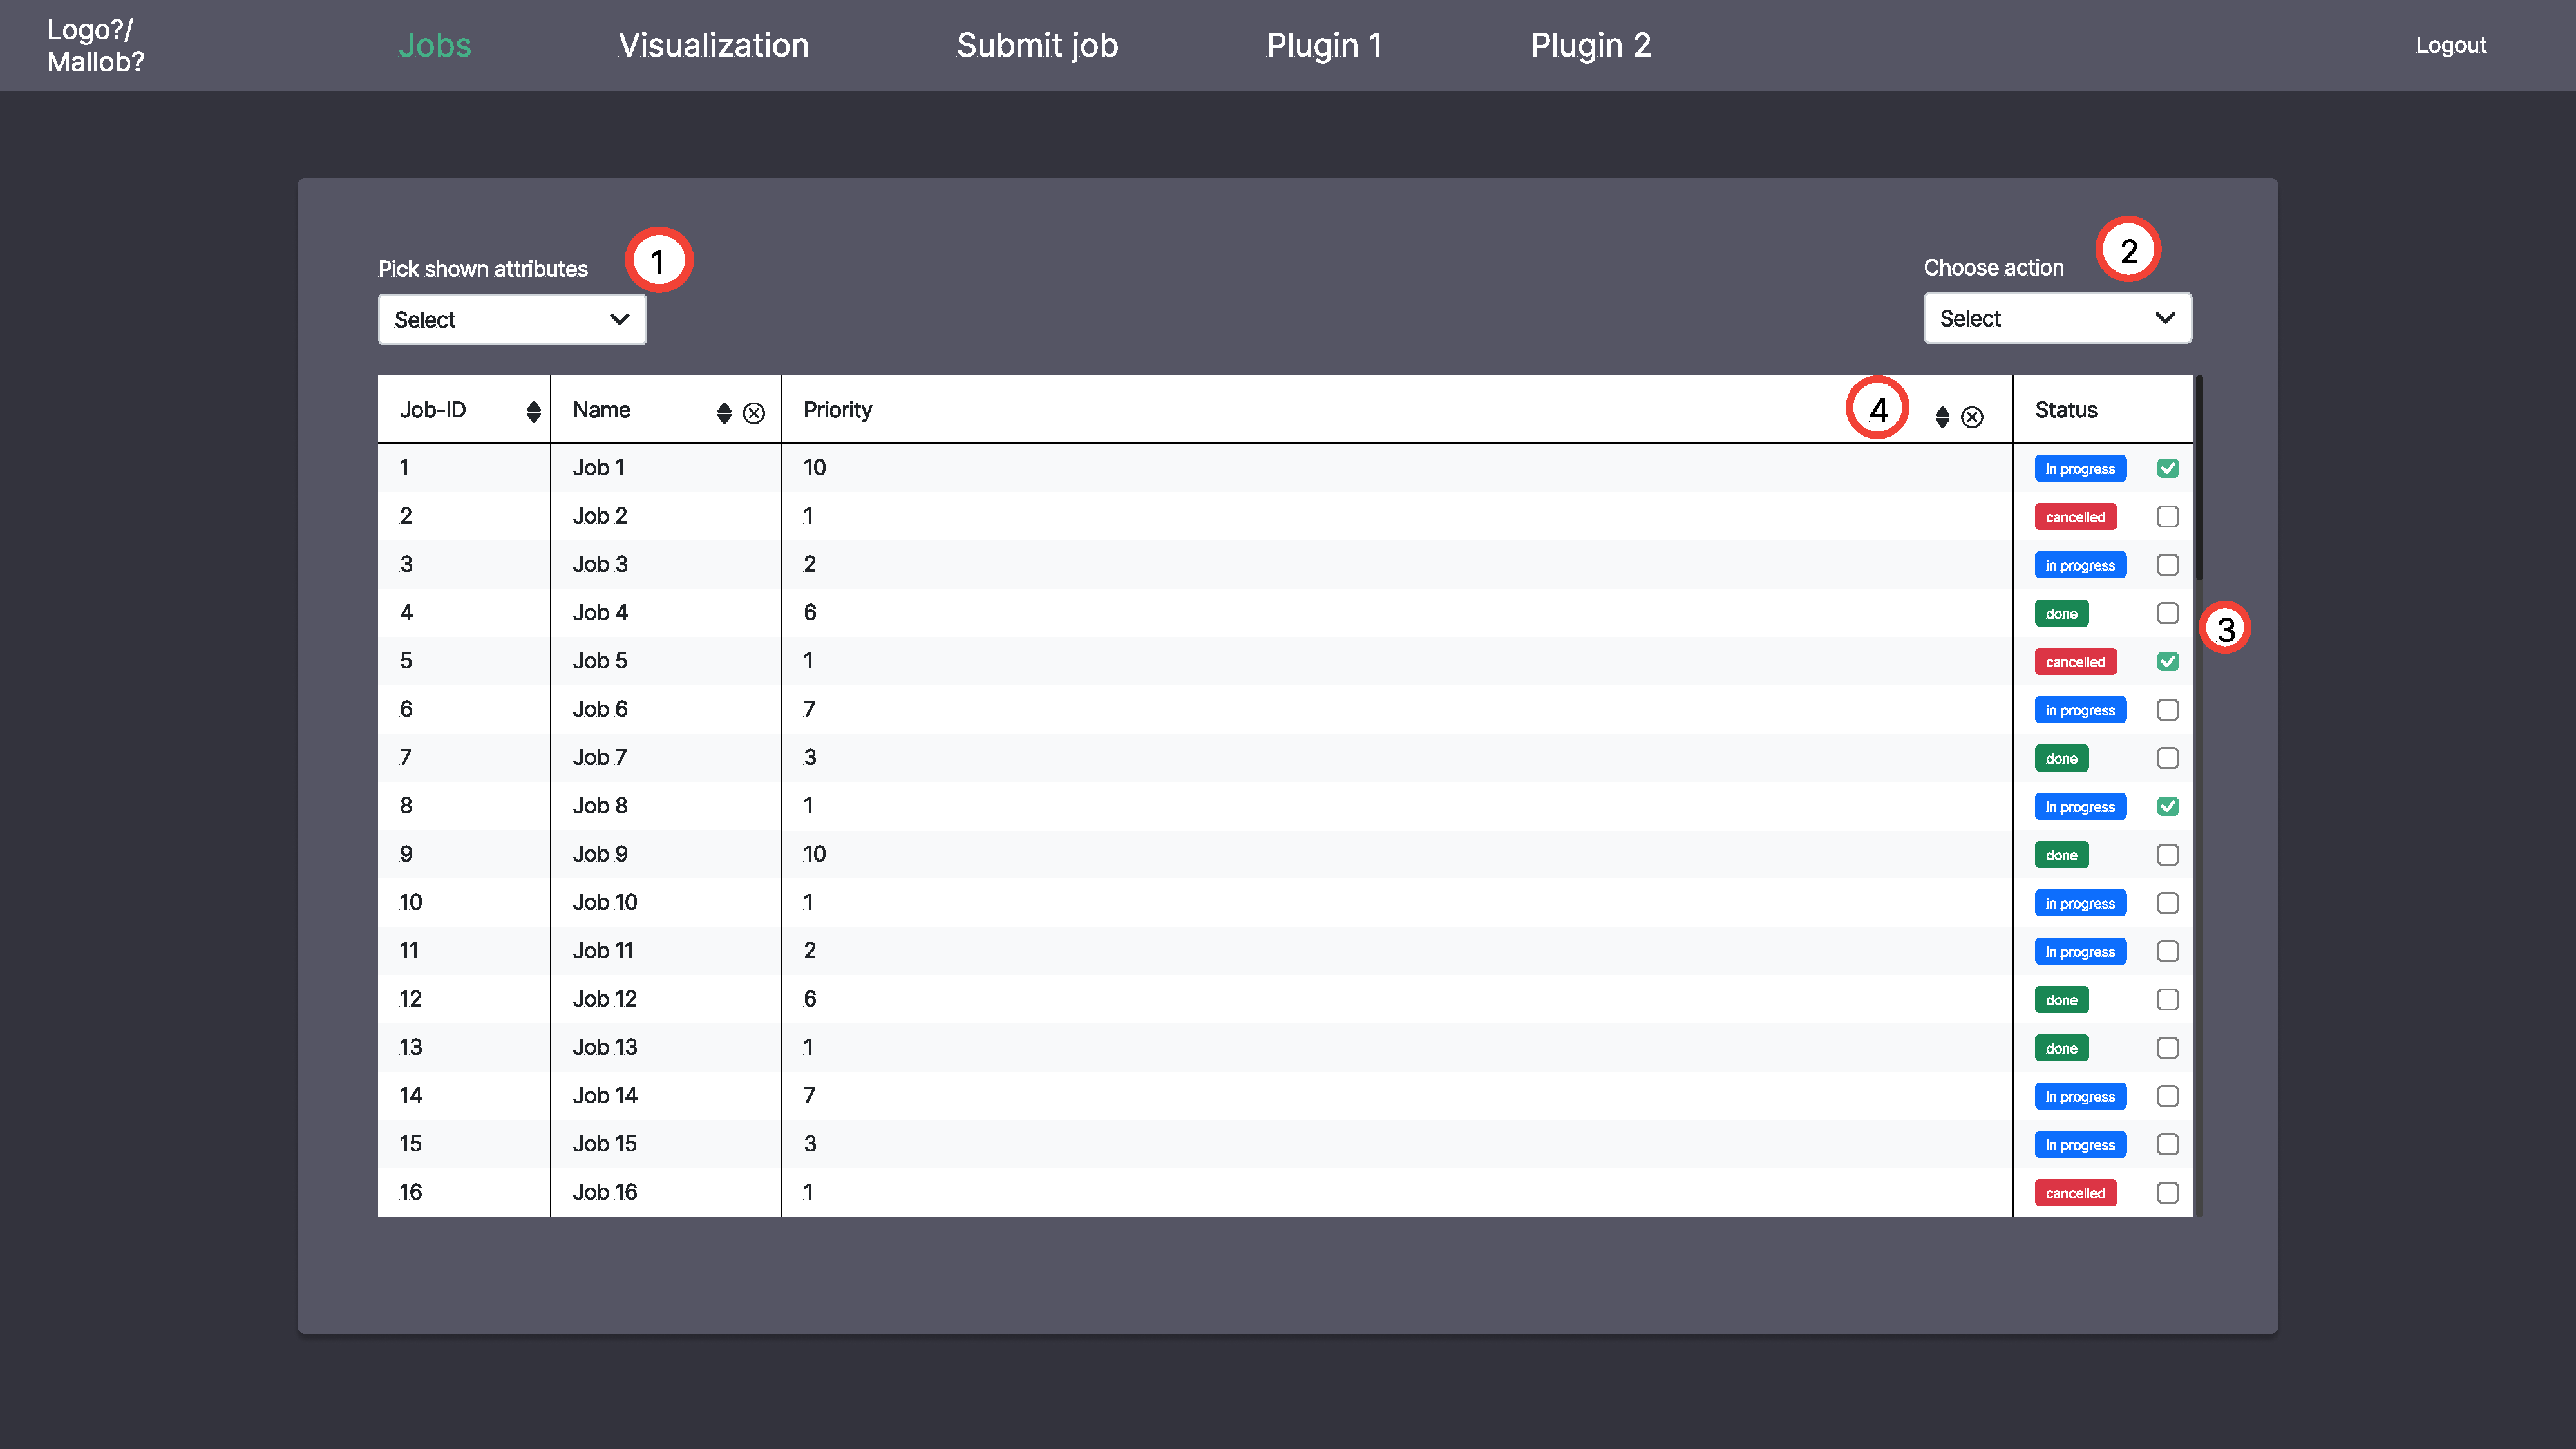
\includegraphics[width=\textwidth]{images-interface/v3_interface/job_table_page_collapsed_v3.pdf}
    \caption{Job—Tabelle}
    \label{fig:job-table-col}

    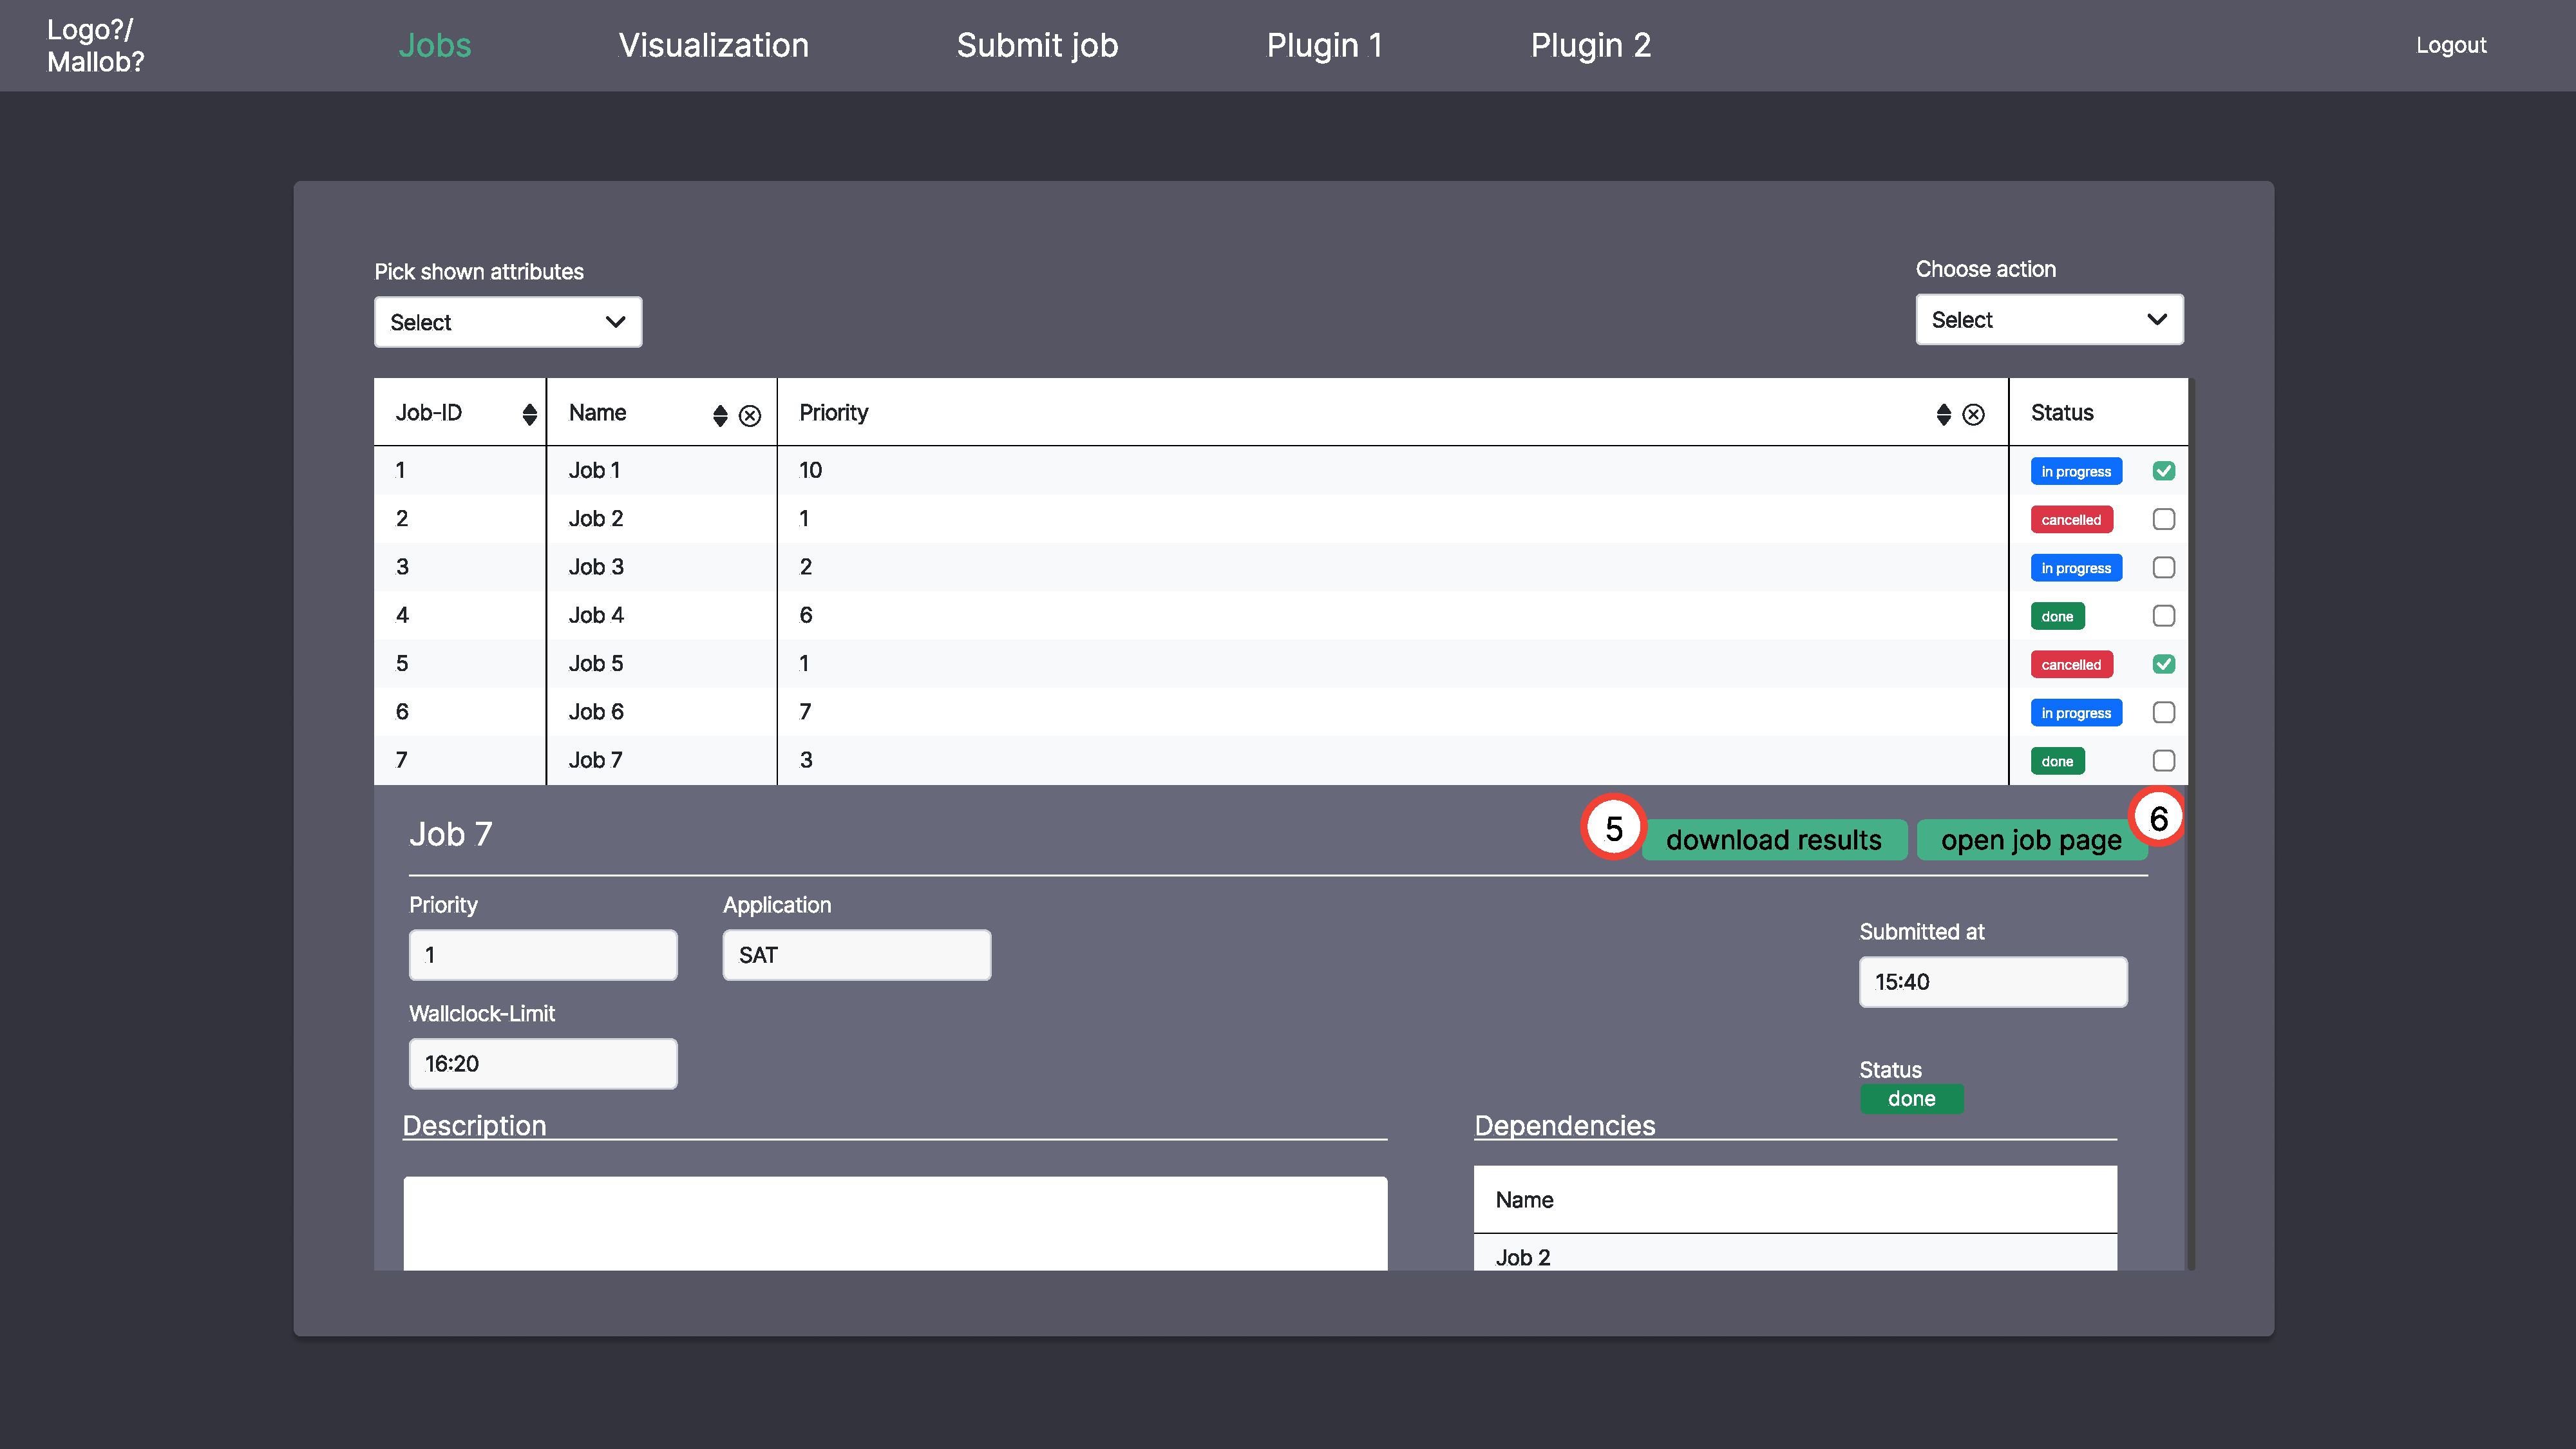
\includegraphics[width=\textwidth]{images-interface/v3_interface/job_table_expanded_v3.pdf}
    \caption{Job-Tabelle mit aufgeklappter Ansicht für einen Job}
    \label{fig:job-table-exp}
\end{figure}

\textbf{Erläuterungen}
\begin{itemize}
    \item[1)] Über dieses Dropdown-Menü können gemäß \hyperref[FA:Web-Interface:Verwalten von Spalten]{FA2120} weitere Attribute in der Tabelle angezeigt werden.
    \item[2)] Über dieses Dropdown-Menü kann eine Aktion (siehe \hyperref[FA:Web-Interface:Abbruch mehrerer Jobs auf einmal]{FA2050} und \hyperref[FA:Web-Interface:herunterladen mehrerer Ergebnisse auf einmal]{FA2070}) durchgeführt werden, welche auf alle mit der Checkbox ausgewählten Jobs angewandt wird.
    \item[3)] Über diese Checkboxen kann ein Job für eine Aktion nach Punkt Zwei dieser Liste ausgewählt werden.
    \item[4)] Über das Symbol mit den beide Dreiecken kann die entsprechende Spalte gemäß \hyperref[FA:Web-Interface:Sortieren der Tabelle]{FA2130} sortiert werden. Mit dem Kreuz-Symbol kann die Spalte wieder aus der Tabelle gelöscht werden.
    \item[5)] Über diese Schaltfläche kann das Ergebnis gemäß \hyperref[FA:Web-Interface:Herunterladen eines einzelnen Ergebnisses]{FA2060} heruntergeladen werden. Man beachte, dass diese Schaltfläche nur bei abgeschlossenen Jobs verfügbar ist. Bei laufenden Jobs bietet sie die Möglichkeit, den Job abzubrechen. Bei abgebrochenen Jobs bietet sie die Möglichkeit, den Job neuzustarten.
    \item[6)] Über diese Schaltfläche wird der Nutzer zur entsprechenden \hyperref[pages:job-page]{Job-Seite} des Jobs weitergeleitet.
\end{itemize}

\newpage
\subsection{Job einreichen}
\label{pages:submit-job}
\begin{figure}[H]
    \centering
    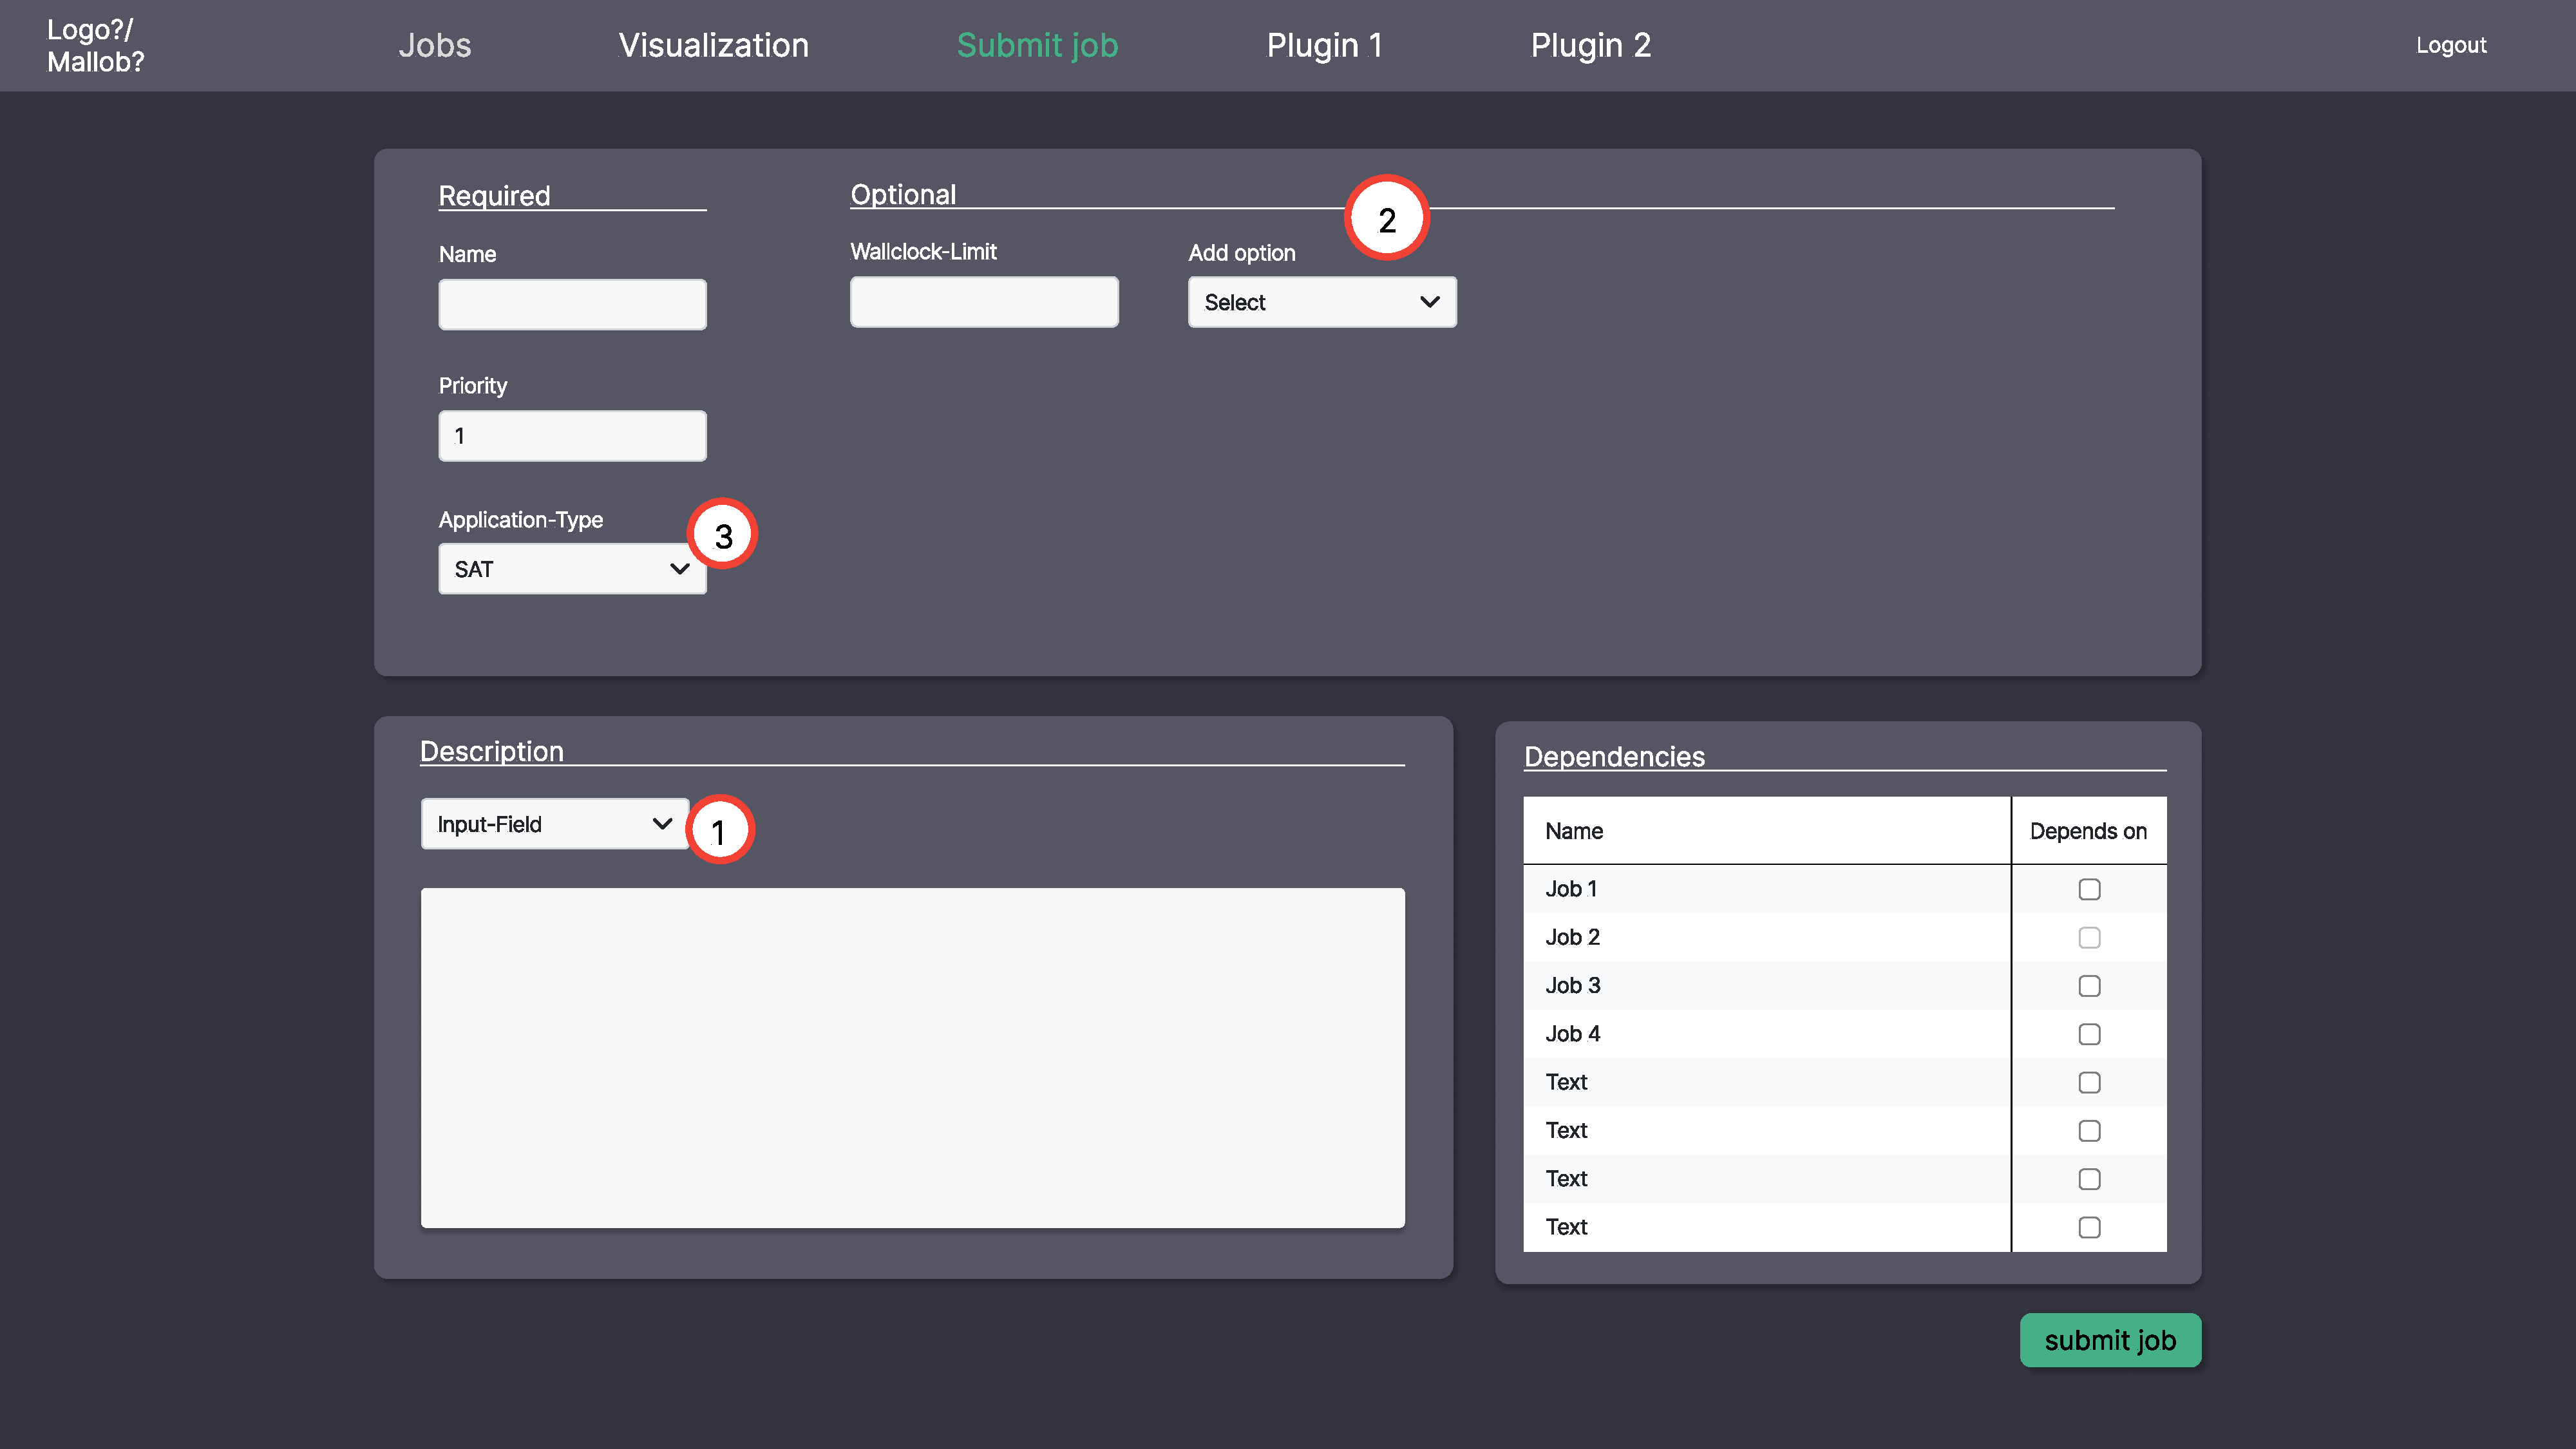
\includegraphics[width=\textwidth]{images-interface/v3_interface/submit_job_page_v3.pdf}
    \caption{Einreichen neuer Jobs}
    \label{fig:submit-job}
\end{figure}
\textbf{Erläuterungen}
\begin{itemize}
    \item[1)] Mit diesem Dropdown-Menü kann gemäß \hyperref[FA:Web-Interface:Job einreichen]{FA2030} gewählt werden, auf welchem Wege die Job-Beschreibung übermittelt wird.
    \item[2)] Mit diesem Dropdown-Menü können weitere, optionale Job-Optionen gemäß \hyperref[FA:Web-Interface:Job einreichen]{FA2030} ausgewählt werden
    \item[3)] Mit diesem Dropdown-Menü kann der Job-Typ ausgewählt werden. Zur Auswahl stehen SAT, DUMMY und KMEANS.
\end{itemize}

\newpage
\subsection{Job-Seite}
\label{pages:job-page}
\begin{figure}[H]
    \centering
    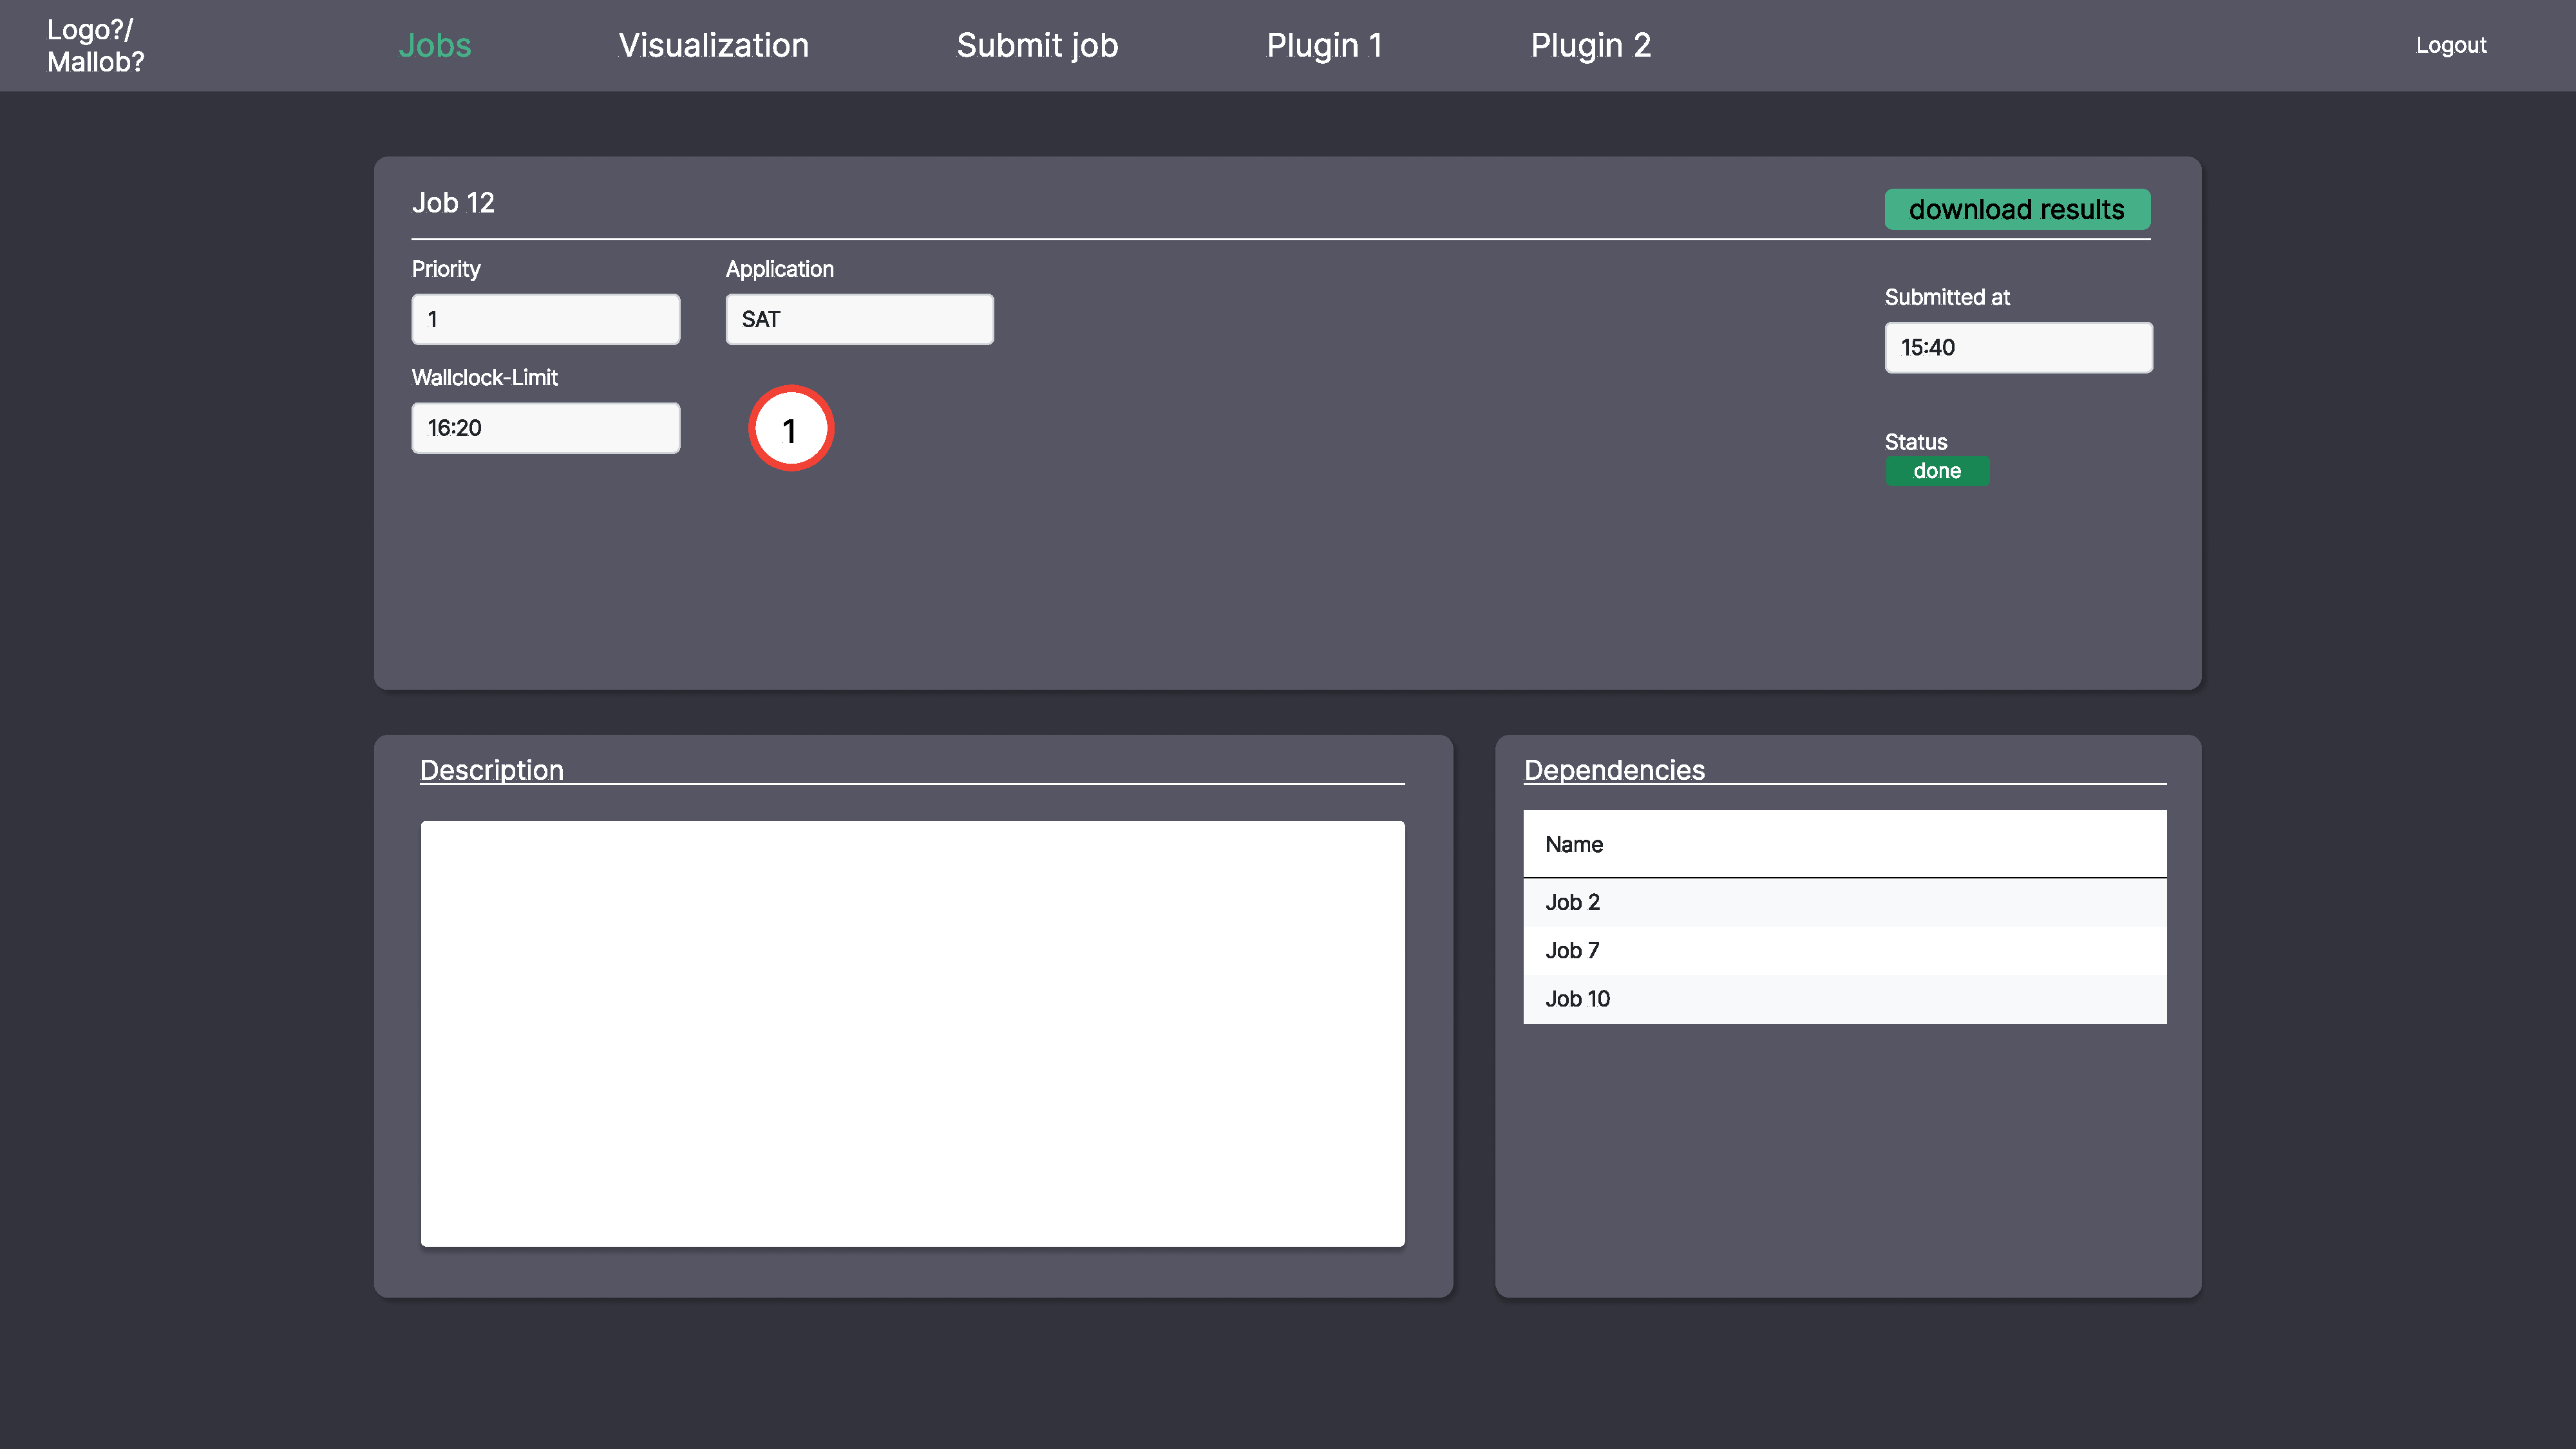
\includegraphics[width=\textwidth]{images-interface/v3_interface/job_info_page_v3.pdf}
    \caption{Info-Seite eines Jobs}
    \label{fig:job-page}
\end{figure}
\begin{itemize}
    \item[1)] Hier werden möglicherweise auch noch weitere, für diesen Job gewählten optionale Optionen angezeigt.
\end{itemize}

\newpage
\subsection{Visualisierung}
\label{pages:visualization}
\begin{figure}[H]
    \centering
    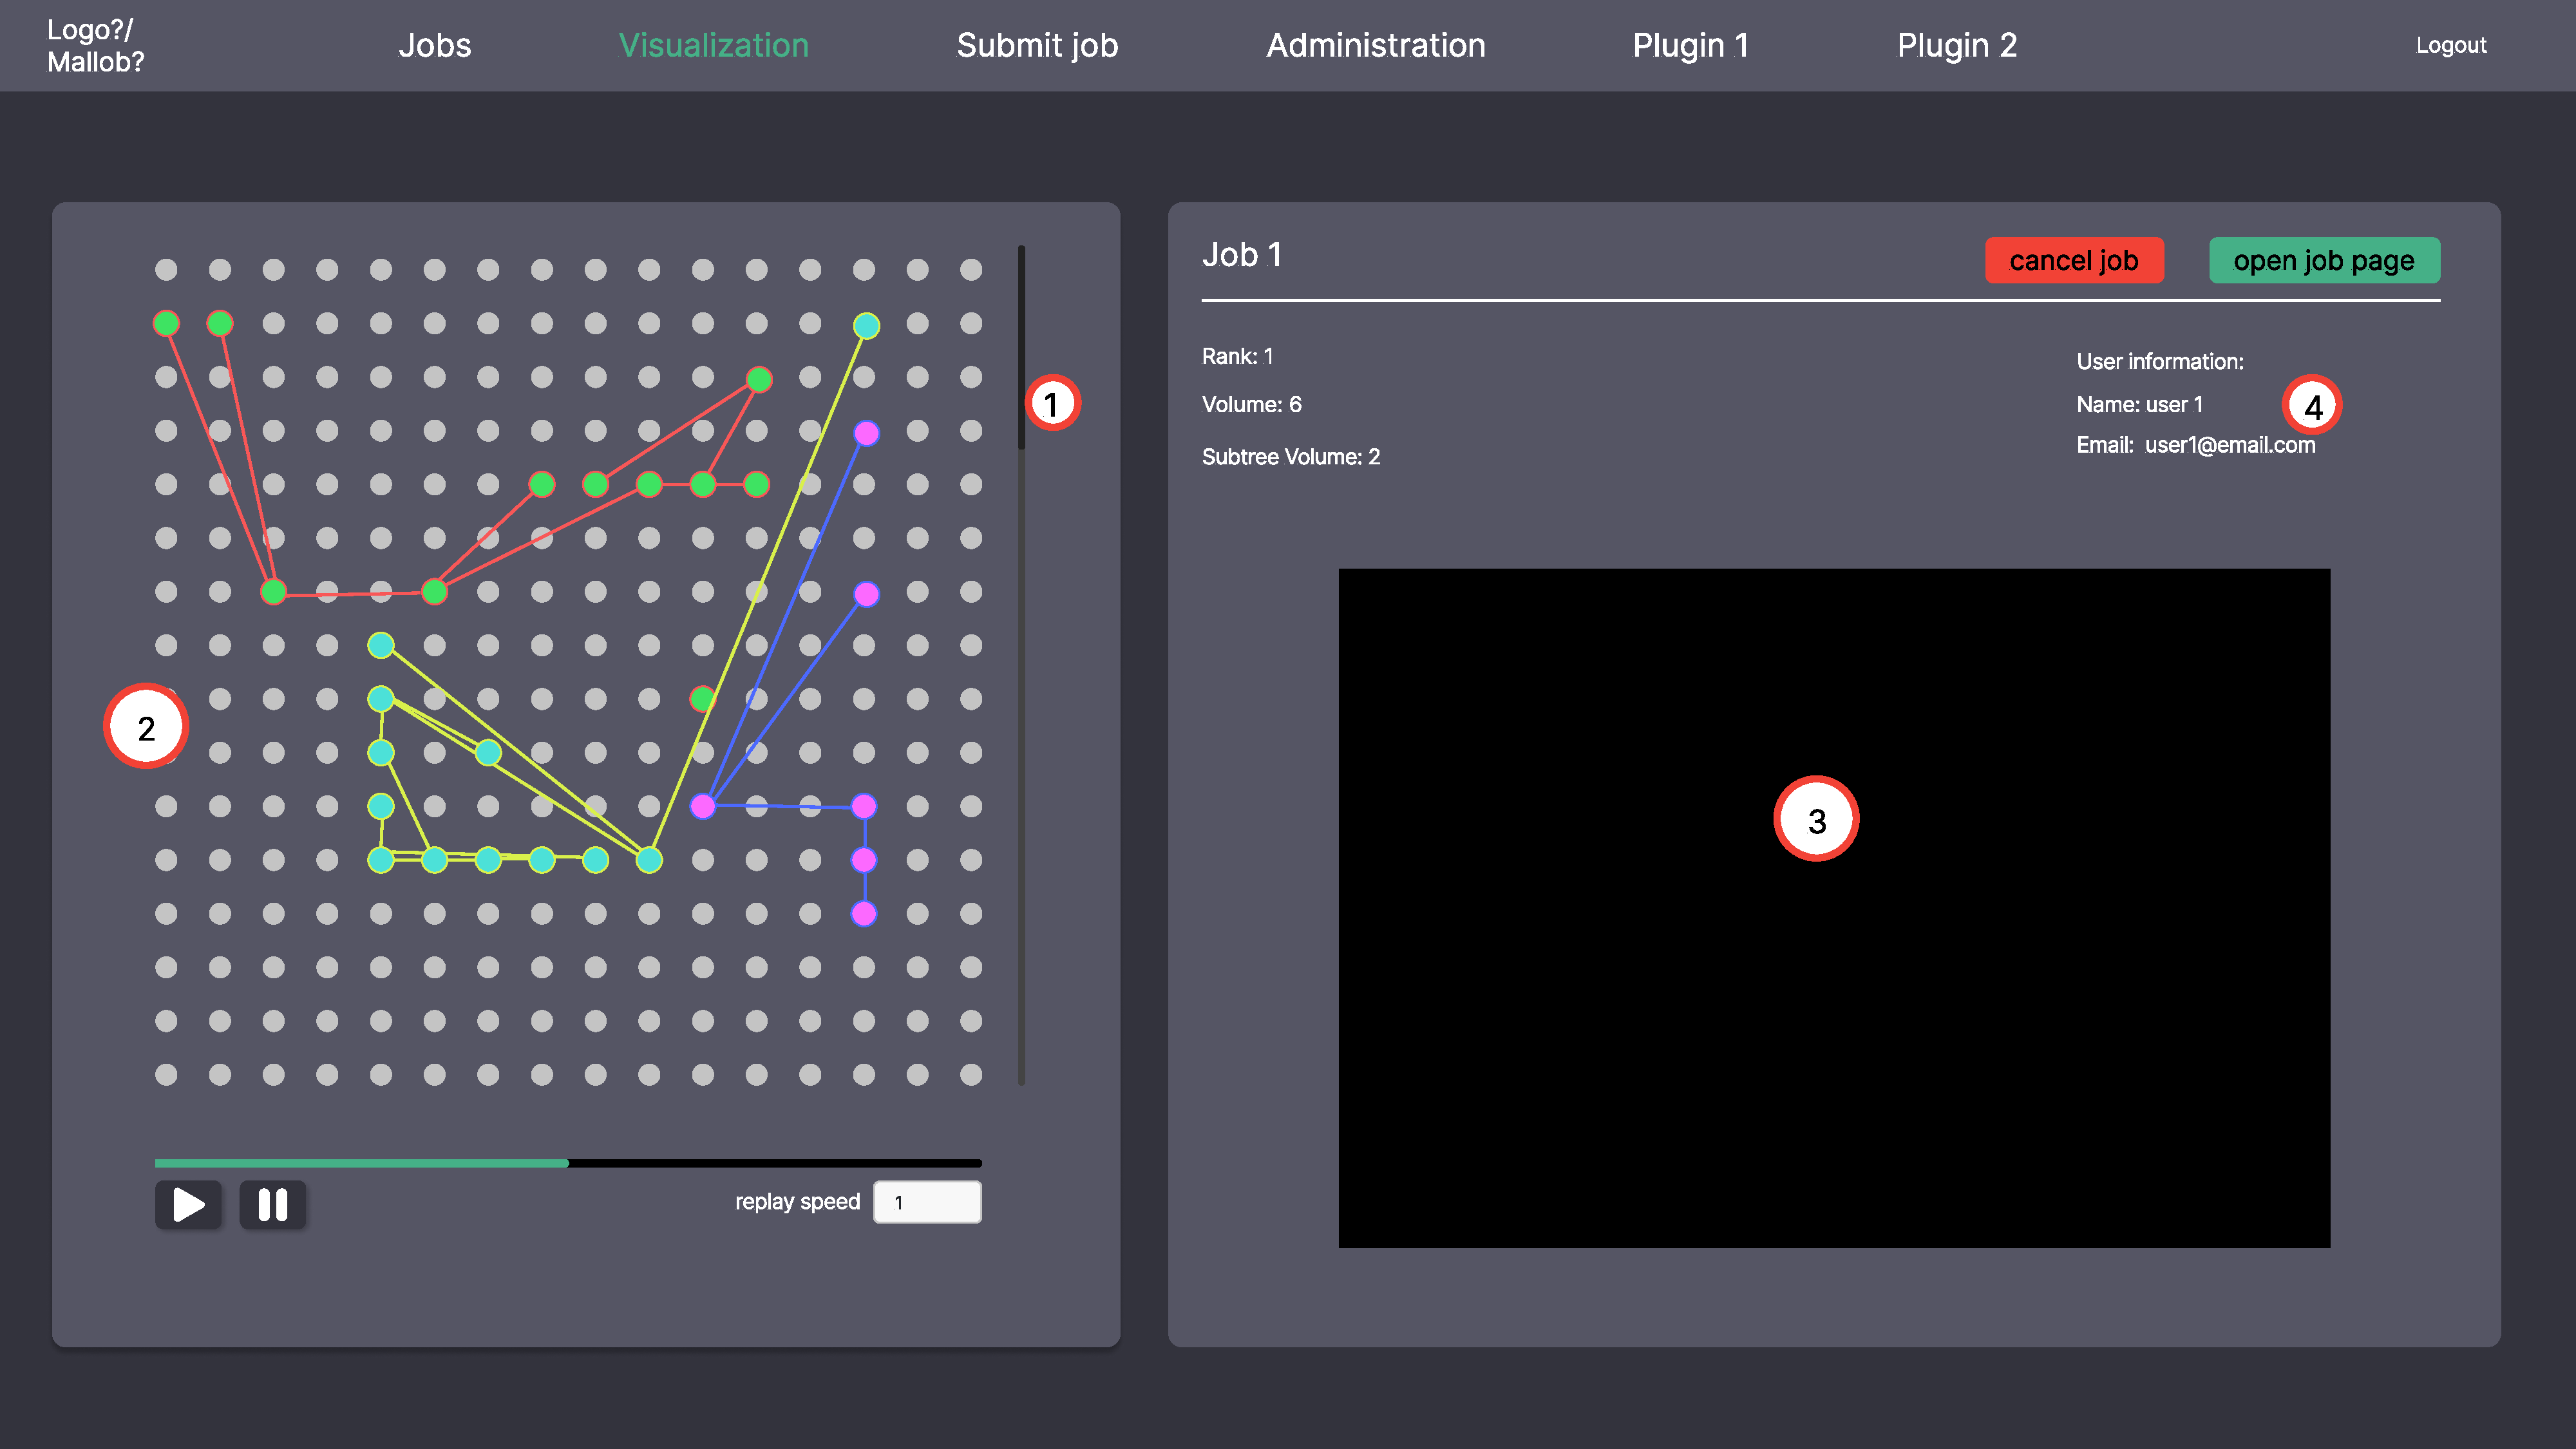
\includegraphics[width=\textwidth]{images-interface/v3_interface/visualization_page_v3.pdf}
    \caption{Visualisierung des Systems}
    \label{fig:visualization-page}
\end{figure}
\begin{itemize}
    \item[1)] Verwendet Mallob zu viele PEs, so erscheint eine Scrollbar, mithilfe die Ansicht vertikal verschoben werden kann.
    \item[2)] Hier findet die eigentliche Visualisierung gemäß \hyperref[FA:Web-Interface:Verifizieren eines Kontos]{FA3000} statt. In diesem Falle ist ein Administrator angemeldet (erkennbar daran, das Schaltfläche "Administration" in der Navigations-Leiste sichbtbar ist), daher sind alle Jobs bunt. Für einen nicht-Administrator werden Jobs von anderen Nutzern pseudonymisiert und grau angezeigt.
    \item[3)] Hier wird gemäß \hyperref[FA:Visualisierung:Anzeigen des Binaerbaumes für einen Job]{FA3010} der Binärbaum eines Jobs angezeigt.
    \item[4)] Informationen über den Nutzer, dem der Job gehört. Wird nur angezeigt, da ein Admin angemeldet ist.
\end{itemize}

%Anmerkung zur Plugin einsicht; Evtl oben in der Querleiste ein Reiter "Plugins" und das dann als Dropdown menü für alle hinzugefügtten Plugins machen. Das macht die Seite stabiler für viele Plguins
% gute idee, schaff ich heute aber nicht mehr

\newpage
\subsection{Plugin-Ansicht}
\label{pages:plugin}
\begin{figure}[H]
    \centering
    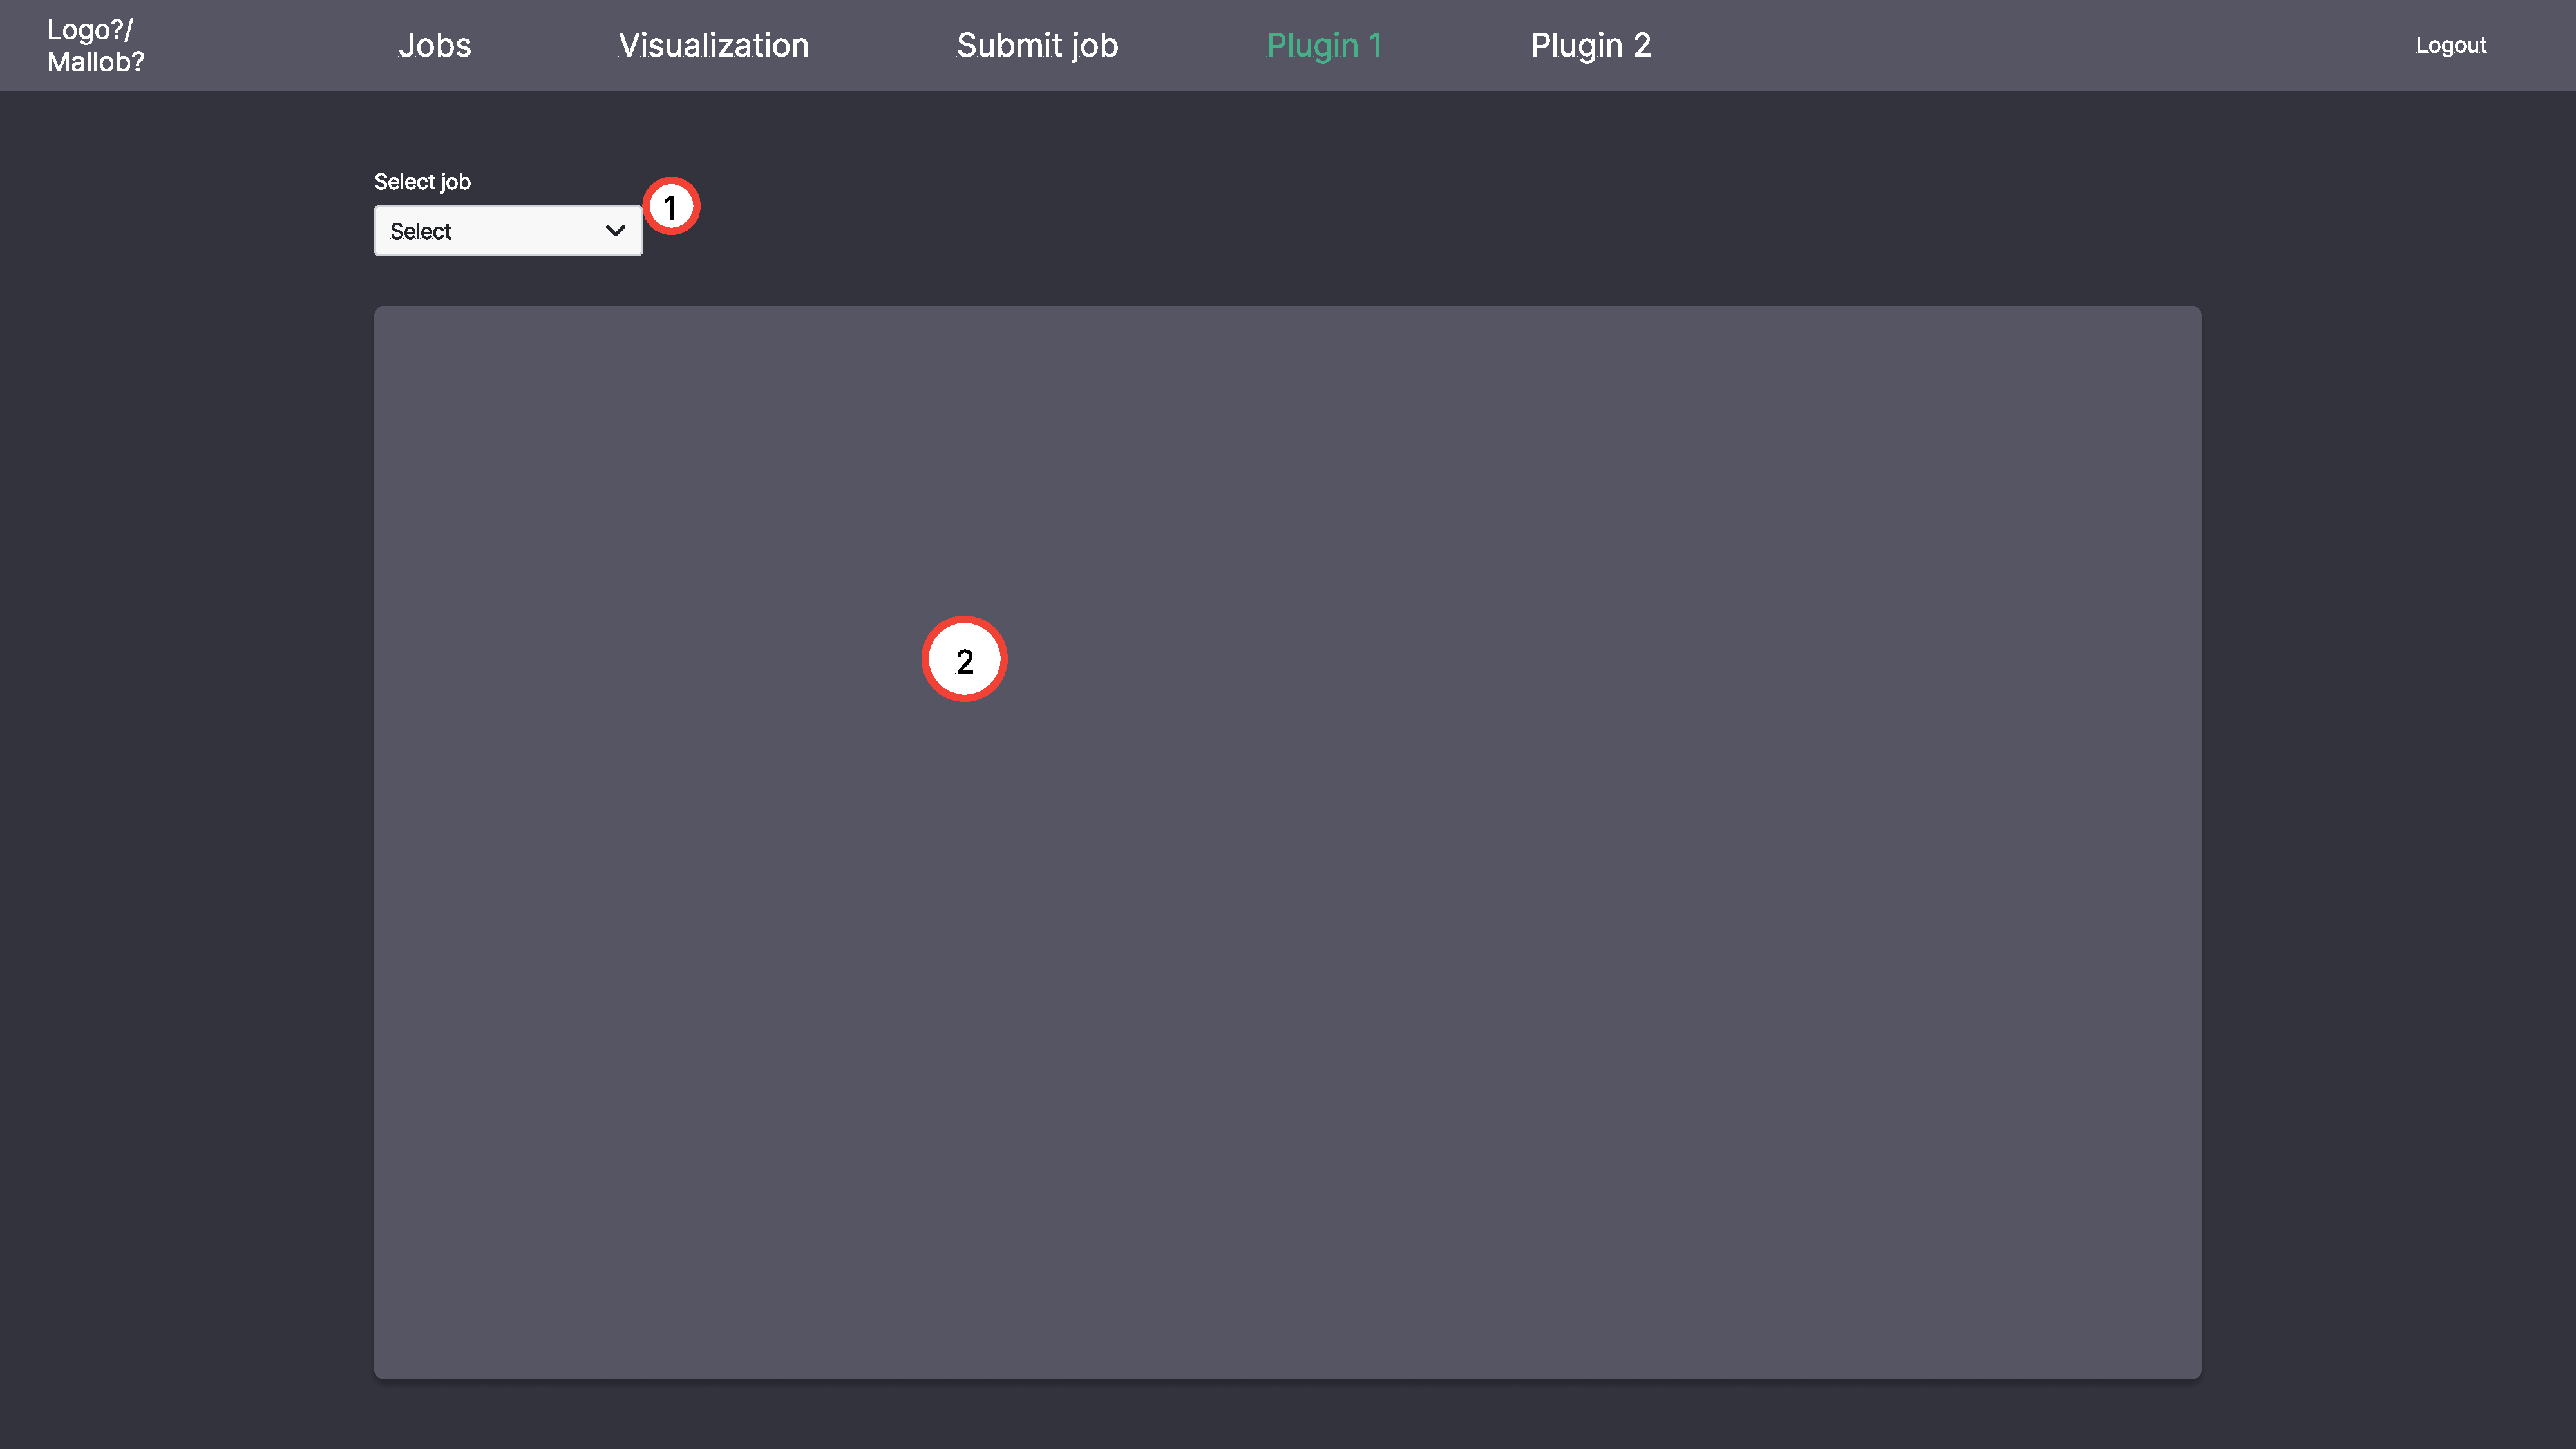
\includegraphics[width=\textwidth]{images-interface/v3_interface/plugin_page_v3.pdf}
    \caption{Generische Ansicht für Plugins}
    \label{fig:plugin-page}
\end{figure}
\begin{itemize}
    \item[1)] Hier kann der Job ausgewählt werden, welcher vom Plugin verarbeitet wird.
    \item[2)] Diese Fläche wird vom entsprechenden Plugin verwendet.
\end{itemize}

\newpage
\subsection{Administration}
\label{pages:admin}
\begin{figure}[H]
    \centering
    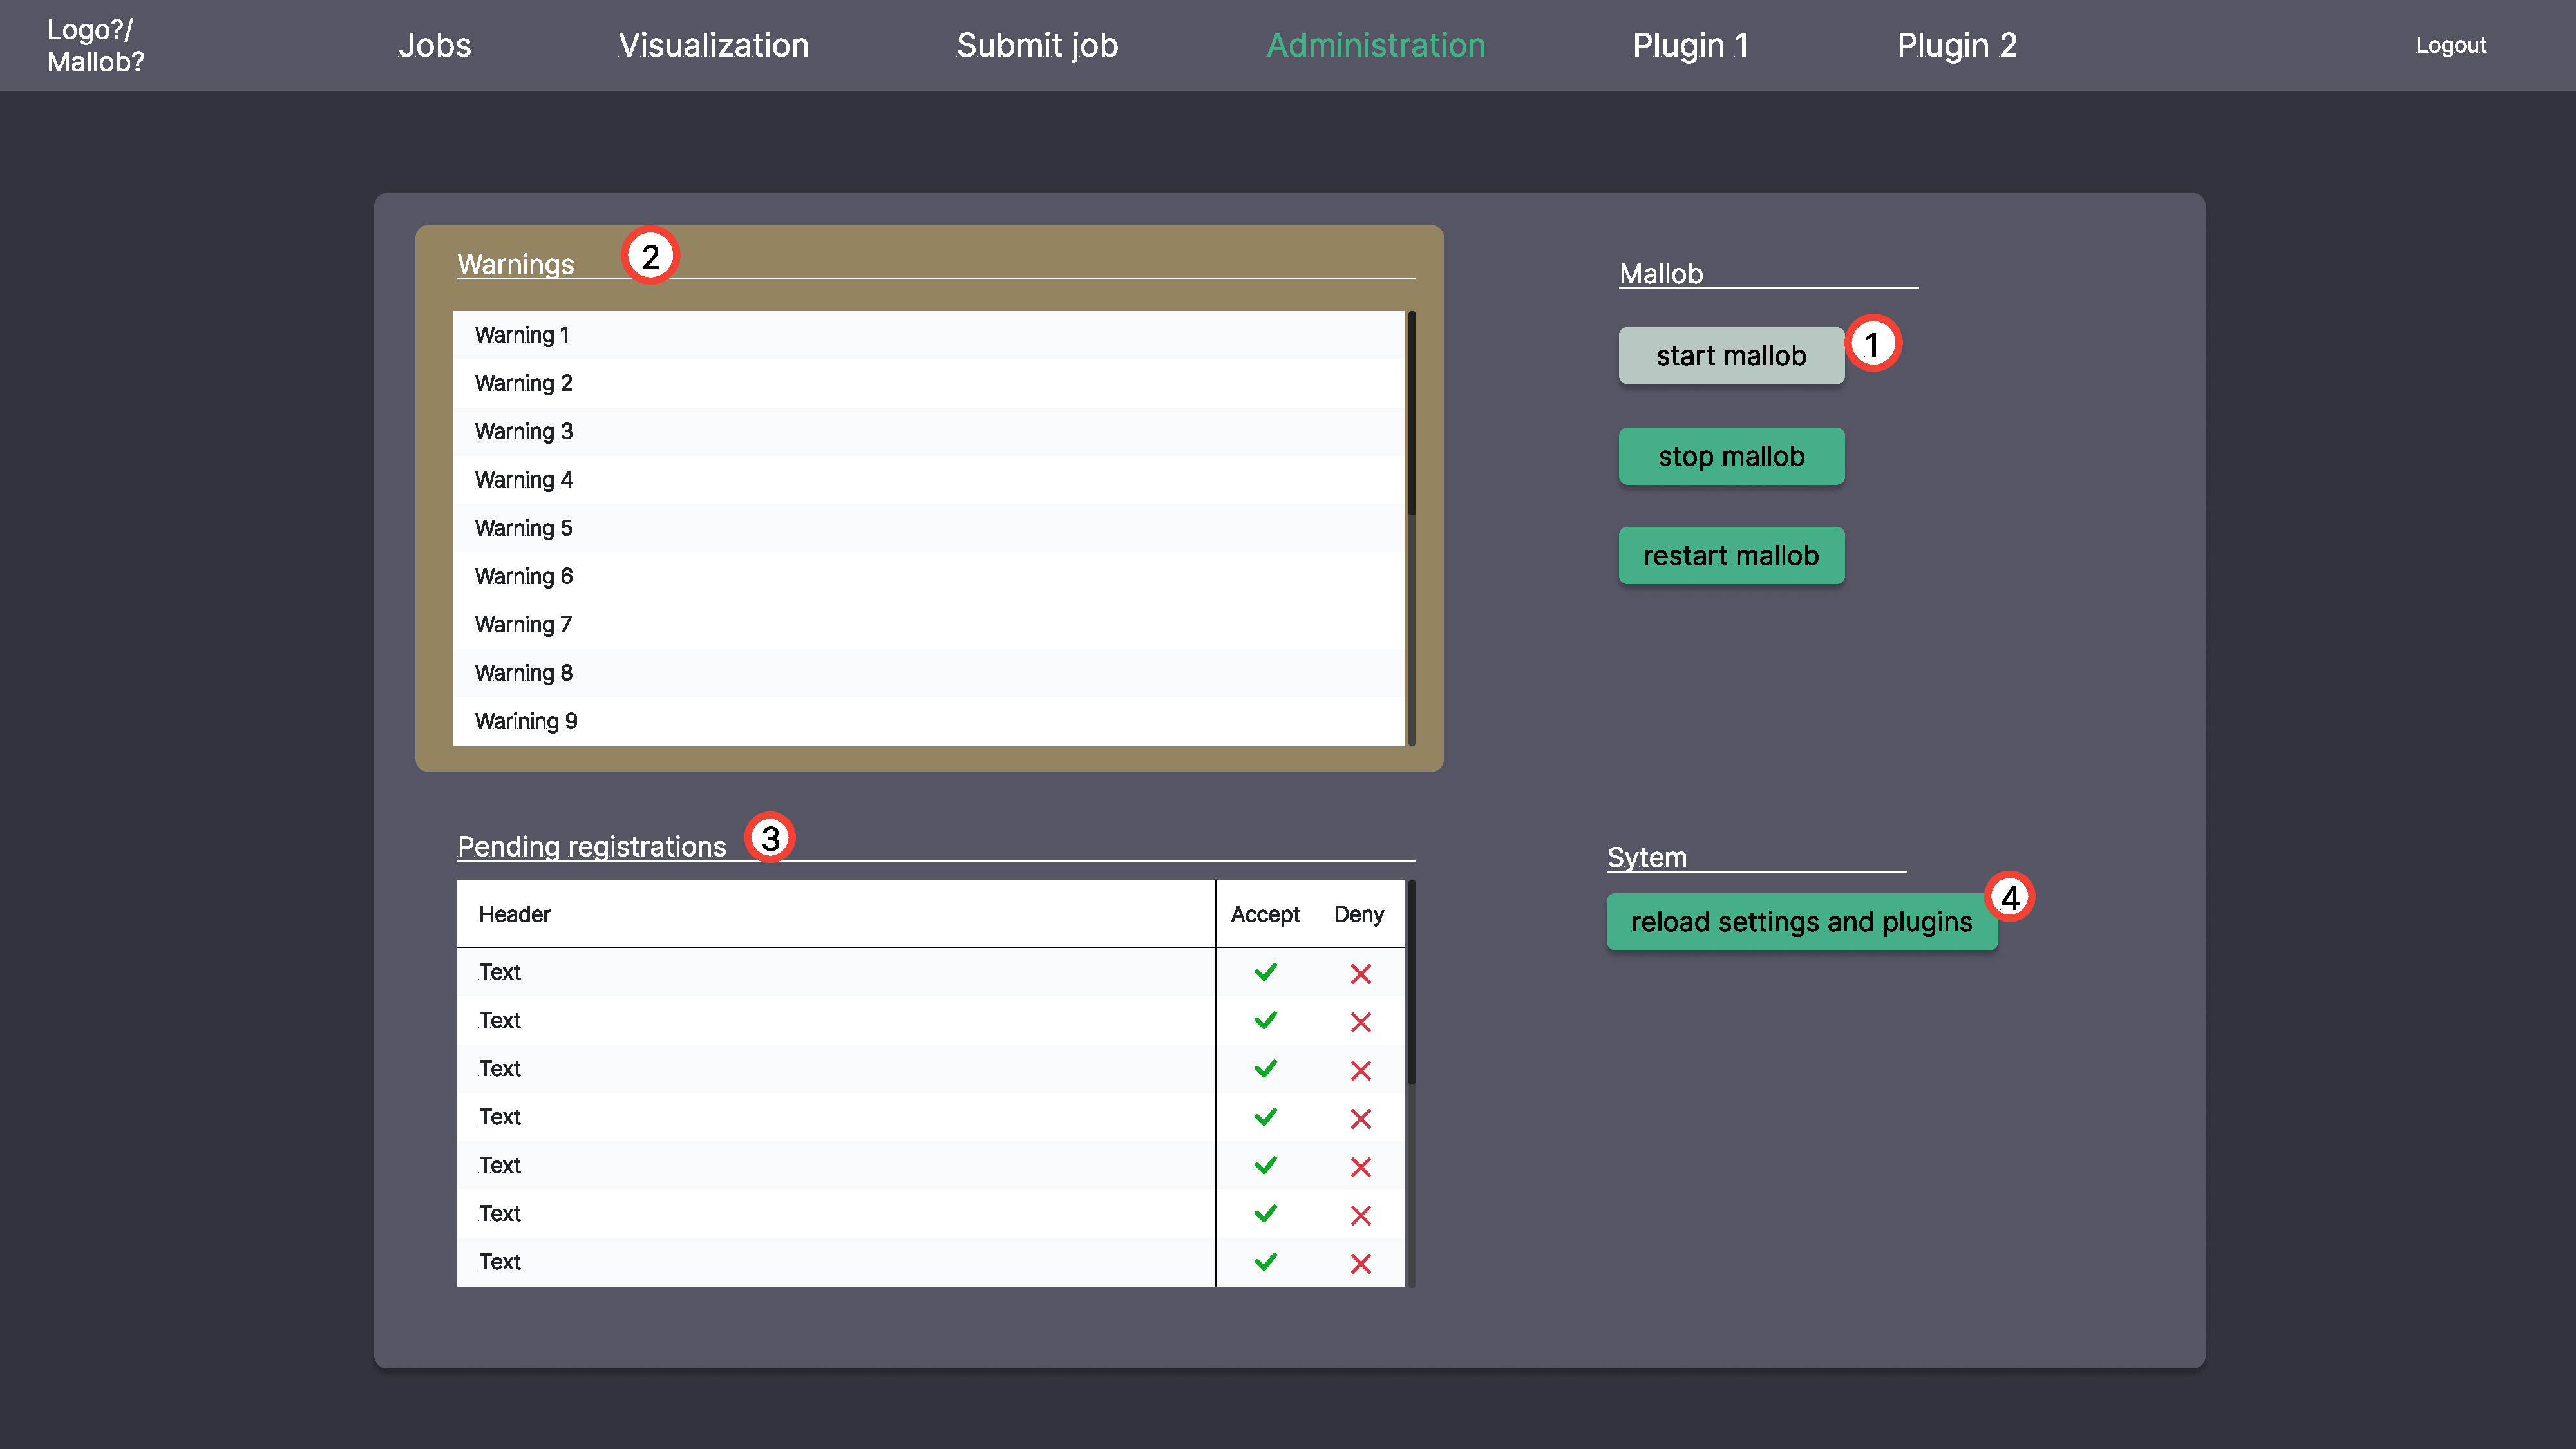
\includegraphics[width=\textwidth]{images-interface/v3_interface/admin_page_v3.pdf}
    \caption{Seite für Administratoren zur Verwaltung}
    \label{fig:admin-page}
\end{figure}
\begin{itemize}
    \item[1)] Hier wird Mallob verwaltet.
    \item[2)] Hier werden gemäß \hyperref[FA:Web-Interface:Anzeigen von Warungen und Fehlermeldungen]{FA2110} Warnungen und Fehlermeldungen angezeigt, die Mallob ausgibt.
    \item[3)] Hier werden gemäß \hyperref[FA:Web-Interface:Verifizieren eines Kontos]{FA2100} nicht verifizierte Konten angezeigt.
    \item[4)] Hier können gemäß \hyperref[FA:Web-Interface:Aktualisieren]{FA2120} die Einstellungen und die Plugins neu geladen werden.
\end{itemize}

%\newpage
%\subsection{Funktionen}
%\begin{itemize}
%    \item /B010/ Es sind zwei Sichten zu unterscheiden: die des Admins, die des Benutzers. 
%    \item /B020/ Benutzer können Funktionen F10, F20, F30 jederzeit nach dem Einloggen aufrufen.
%    \item /B030/ Jeder Benutzer fängt auf der Login/Register-Seite an.
%    \item /B040/ Sobald der Benutzer eingeloggt wird, sieht er die Startseite.
%    \item /B050/ Jeder Nutzer kann seine Jobs anhand der Aufwand auf das Kern unterscheiden (z.B Farbe, Größe usw.)
%    \item /B060/ Admins können alle Funktionen, die die Benutzer können.
%    \item /B070/ Unterschiedliche Benutzer und ihre Befugnisse sollen entsprechend behandelt werden (nicht-funktionale Anforderung?).
%    \item /B080/ Die Bedienungsoberfläche ist auf Mausbedienung auszulegen; eine Bedienung ohne Maus muss aber auch möglich sein. ([TODO] Bediengung ohne Maus auf jeden Fall wunschkriterium oder vlt sogar gar nicth, auf jeden Fall mal fragen, hört sich kompliziert und nicht wirklich notwendig an)
%\end{itemize}